% Options for packages loaded elsewhere
\PassOptionsToPackage{unicode}{hyperref}
\PassOptionsToPackage{hyphens}{url}
%
\documentclass[
]{article}
\usepackage{amsmath,amssymb}
\usepackage{iftex}
\ifPDFTeX
  \usepackage[T1]{fontenc}
  \usepackage[utf8]{inputenc}
  \usepackage{textcomp} % provide euro and other symbols
\else % if luatex or xetex
  \usepackage{unicode-math} % this also loads fontspec
  \defaultfontfeatures{Scale=MatchLowercase}
  \defaultfontfeatures[\rmfamily]{Ligatures=TeX,Scale=1}
\fi
\usepackage{lmodern}
\ifPDFTeX\else
  % xetex/luatex font selection
\fi
% Use upquote if available, for straight quotes in verbatim environments
\IfFileExists{upquote.sty}{\usepackage{upquote}}{}
\IfFileExists{microtype.sty}{% use microtype if available
  \usepackage[]{microtype}
  \UseMicrotypeSet[protrusion]{basicmath} % disable protrusion for tt fonts
}{}
\makeatletter
\@ifundefined{KOMAClassName}{% if non-KOMA class
  \IfFileExists{parskip.sty}{%
    \usepackage{parskip}
  }{% else
    \setlength{\parindent}{0pt}
    \setlength{\parskip}{6pt plus 2pt minus 1pt}}
}{% if KOMA class
  \KOMAoptions{parskip=half}}
\makeatother
\usepackage{xcolor}
\usepackage[margin=1in]{geometry}
\usepackage{color}
\usepackage{fancyvrb}
\newcommand{\VerbBar}{|}
\newcommand{\VERB}{\Verb[commandchars=\\\{\}]}
\DefineVerbatimEnvironment{Highlighting}{Verbatim}{commandchars=\\\{\}}
% Add ',fontsize=\small' for more characters per line
\usepackage{framed}
\definecolor{shadecolor}{RGB}{248,248,248}
\newenvironment{Shaded}{\begin{snugshade}}{\end{snugshade}}
\newcommand{\AlertTok}[1]{\textcolor[rgb]{0.94,0.16,0.16}{#1}}
\newcommand{\AnnotationTok}[1]{\textcolor[rgb]{0.56,0.35,0.01}{\textbf{\textit{#1}}}}
\newcommand{\AttributeTok}[1]{\textcolor[rgb]{0.13,0.29,0.53}{#1}}
\newcommand{\BaseNTok}[1]{\textcolor[rgb]{0.00,0.00,0.81}{#1}}
\newcommand{\BuiltInTok}[1]{#1}
\newcommand{\CharTok}[1]{\textcolor[rgb]{0.31,0.60,0.02}{#1}}
\newcommand{\CommentTok}[1]{\textcolor[rgb]{0.56,0.35,0.01}{\textit{#1}}}
\newcommand{\CommentVarTok}[1]{\textcolor[rgb]{0.56,0.35,0.01}{\textbf{\textit{#1}}}}
\newcommand{\ConstantTok}[1]{\textcolor[rgb]{0.56,0.35,0.01}{#1}}
\newcommand{\ControlFlowTok}[1]{\textcolor[rgb]{0.13,0.29,0.53}{\textbf{#1}}}
\newcommand{\DataTypeTok}[1]{\textcolor[rgb]{0.13,0.29,0.53}{#1}}
\newcommand{\DecValTok}[1]{\textcolor[rgb]{0.00,0.00,0.81}{#1}}
\newcommand{\DocumentationTok}[1]{\textcolor[rgb]{0.56,0.35,0.01}{\textbf{\textit{#1}}}}
\newcommand{\ErrorTok}[1]{\textcolor[rgb]{0.64,0.00,0.00}{\textbf{#1}}}
\newcommand{\ExtensionTok}[1]{#1}
\newcommand{\FloatTok}[1]{\textcolor[rgb]{0.00,0.00,0.81}{#1}}
\newcommand{\FunctionTok}[1]{\textcolor[rgb]{0.13,0.29,0.53}{\textbf{#1}}}
\newcommand{\ImportTok}[1]{#1}
\newcommand{\InformationTok}[1]{\textcolor[rgb]{0.56,0.35,0.01}{\textbf{\textit{#1}}}}
\newcommand{\KeywordTok}[1]{\textcolor[rgb]{0.13,0.29,0.53}{\textbf{#1}}}
\newcommand{\NormalTok}[1]{#1}
\newcommand{\OperatorTok}[1]{\textcolor[rgb]{0.81,0.36,0.00}{\textbf{#1}}}
\newcommand{\OtherTok}[1]{\textcolor[rgb]{0.56,0.35,0.01}{#1}}
\newcommand{\PreprocessorTok}[1]{\textcolor[rgb]{0.56,0.35,0.01}{\textit{#1}}}
\newcommand{\RegionMarkerTok}[1]{#1}
\newcommand{\SpecialCharTok}[1]{\textcolor[rgb]{0.81,0.36,0.00}{\textbf{#1}}}
\newcommand{\SpecialStringTok}[1]{\textcolor[rgb]{0.31,0.60,0.02}{#1}}
\newcommand{\StringTok}[1]{\textcolor[rgb]{0.31,0.60,0.02}{#1}}
\newcommand{\VariableTok}[1]{\textcolor[rgb]{0.00,0.00,0.00}{#1}}
\newcommand{\VerbatimStringTok}[1]{\textcolor[rgb]{0.31,0.60,0.02}{#1}}
\newcommand{\WarningTok}[1]{\textcolor[rgb]{0.56,0.35,0.01}{\textbf{\textit{#1}}}}
\usepackage{graphicx}
\makeatletter
\def\maxwidth{\ifdim\Gin@nat@width>\linewidth\linewidth\else\Gin@nat@width\fi}
\def\maxheight{\ifdim\Gin@nat@height>\textheight\textheight\else\Gin@nat@height\fi}
\makeatother
% Scale images if necessary, so that they will not overflow the page
% margins by default, and it is still possible to overwrite the defaults
% using explicit options in \includegraphics[width, height, ...]{}
\setkeys{Gin}{width=\maxwidth,height=\maxheight,keepaspectratio}
% Set default figure placement to htbp
\makeatletter
\def\fps@figure{htbp}
\makeatother
\setlength{\emergencystretch}{3em} % prevent overfull lines
\providecommand{\tightlist}{%
  \setlength{\itemsep}{0pt}\setlength{\parskip}{0pt}}
\setcounter{secnumdepth}{-\maxdimen} % remove section numbering
\usepackage{fvextra}
\DefineVerbatimEnvironment{Highlighting}{Verbatim}{
  breaklines,           % activa saltos de línea
  breakanywhere=true,   % permite romper donde sea
  commandchars=\\\{\}, 
  fontsize=\small,      % tamaño del código
  tabsize=2,            % tamaño de tabulación
  frame=single          % marco opcional (puedes quitarlo)
}
\ifLuaTeX
  \usepackage{selnolig}  % disable illegal ligatures
\fi
\IfFileExists{bookmark.sty}{\usepackage{bookmark}}{\usepackage{hyperref}}
\IfFileExists{xurl.sty}{\usepackage{xurl}}{} % add URL line breaks if available
\urlstyle{same}
\hypersetup{
  pdftitle={Informe sobre ``Experiencia con el uso de  a través de  en el Grado en Biología''},
  hidelinks,
  pdfcreator={LaTeX via pandoc}}

\title{Informe sobre ``Experiencia con el uso de \texttt{R Markdown} a
través de \texttt{R-Commander} en el Grado en Biología''}
\author{\Large Miguel Ángel Beltrán-Sánchez\(^1\), Adina Iftimi\(^2\), y
Gabriel Calvo-Bayarri\(^3\)\\
\(^1\)\href{mailto:angel.beltran@uv.es}{\nolinkurl{angel.beltran@uv.es}};
\(^2\)\href{mailto:adina.iftimi@uv.es}{\nolinkurl{adina.iftimi@uv.es}};
\(^3\)\href{mailto:gabriel.calvo@uv.es}{\nolinkurl{gabriel.calvo@uv.es}}\\
Departamento de Estadística e Investigación Operativa\\
Facultad de Ciencias Matemáticas, Universidad de Valencia}
\date{}

\begin{document}
\maketitle

\hypertarget{paquetes-requeridos}{%
\section{Paquetes requeridos}\label{paquetes-requeridos}}

\begin{Shaded}
\begin{Highlighting}[]
\DocumentationTok{\#\# install.packages("pacman")}

\NormalTok{pacman}\SpecialCharTok{::}\FunctionTok{p\_load}\NormalTok{(readxl, ggplot2, graphics, wordcloud, tm, }\AttributeTok{install =} \ConstantTok{FALSE}\NormalTok{)}
\end{Highlighting}
\end{Shaded}

\hypertarget{carga-de-datos}{%
\section{Carga de datos}\label{carga-de-datos}}

\begin{Shaded}
\begin{Highlighting}[]
\FunctionTok{rm}\NormalTok{(}\AttributeTok{list =} \FunctionTok{ls}\NormalTok{())}
\NormalTok{encuesta }\OtherTok{\textless{}{-}} \FunctionTok{read\_excel}\NormalTok{(}\FunctionTok{file.path}\NormalTok{(}\StringTok{".."}\NormalTok{, }\StringTok{"data"}\NormalTok{, }\StringTok{"EncuestaRMD2025.xlsx"}\NormalTok{), }\AttributeTok{col\_names =} \ConstantTok{TRUE}\NormalTok{)}

\NormalTok{encuesta}\SpecialCharTok{$}\NormalTok{P0 }\OtherTok{\textless{}{-}} \FunctionTok{factor}\NormalTok{(encuesta}\SpecialCharTok{$}\NormalTok{P0, }\AttributeTok{levels =} \FunctionTok{c}\NormalTok{(}\StringTok{"Castellano"}\NormalTok{, }\StringTok{"Valenciano"}\NormalTok{))}
\NormalTok{encuesta}\SpecialCharTok{$}\NormalTok{P1 }\OtherTok{\textless{}{-}} \FunctionTok{factor}\NormalTok{(encuesta}\SpecialCharTok{$}\NormalTok{P1, }\AttributeTok{levels =} \FunctionTok{c}\NormalTok{(}\StringTok{"BI1"}\NormalTok{, }\StringTok{"BI2"}\NormalTok{, }\StringTok{"AI1"}\NormalTok{, }\StringTok{"AI2"}\NormalTok{))}
\NormalTok{encuesta}\SpecialCharTok{$}\NormalTok{P2 }\OtherTok{\textless{}{-}} \FunctionTok{factor}\NormalTok{(encuesta}\SpecialCharTok{$}\NormalTok{P2, }\AttributeTok{levels =} \FunctionTok{c}\NormalTok{(}\StringTok{"No"}\NormalTok{, }\StringTok{"Si"}\NormalTok{))}
\NormalTok{encuesta}\SpecialCharTok{$}\NormalTok{P3 }\OtherTok{\textless{}{-}} \FunctionTok{factor}\NormalTok{(encuesta}\SpecialCharTok{$}\NormalTok{P3, }\AttributeTok{levels =} \FunctionTok{c}\NormalTok{(}\StringTok{"No"}\NormalTok{, }\StringTok{"Si"}\NormalTok{))}
\NormalTok{encuesta}\SpecialCharTok{$}\NormalTok{P4 }\OtherTok{\textless{}{-}} \FunctionTok{factor}\NormalTok{(encuesta}\SpecialCharTok{$}\NormalTok{P4, }\AttributeTok{levels =} \FunctionTok{c}\NormalTok{(}\StringTok{"No"}\NormalTok{, }\StringTok{"Si"}\NormalTok{))}
\NormalTok{encuesta}\SpecialCharTok{$}\NormalTok{P5 }\OtherTok{\textless{}{-}} \FunctionTok{factor}\NormalTok{(encuesta}\SpecialCharTok{$}\NormalTok{P5, }\AttributeTok{levels =} \FunctionTok{c}\NormalTok{(}\StringTok{"No"}\NormalTok{, }\StringTok{"Si"}\NormalTok{))}
\NormalTok{encuesta}\SpecialCharTok{$}\NormalTok{P6 }\OtherTok{\textless{}{-}} \FunctionTok{factor}\NormalTok{(encuesta}\SpecialCharTok{$}\NormalTok{P6, }\AttributeTok{levels =} \FunctionTok{c}\NormalTok{(}\StringTok{"No"}\NormalTok{, }\StringTok{"Si"}\NormalTok{))}
\NormalTok{encuesta}\SpecialCharTok{$}\NormalTok{P7 }\OtherTok{\textless{}{-}} \FunctionTok{factor}\NormalTok{(encuesta}\SpecialCharTok{$}\NormalTok{P7, }\AttributeTok{levels =} \FunctionTok{c}\NormalTok{(}\StringTok{"Muy facil"}\NormalTok{, }\StringTok{"Facil"}\NormalTok{, }\StringTok{"Normal"}\NormalTok{, }\StringTok{"Dificil"}\NormalTok{, }\StringTok{"Muy dificil"}\NormalTok{))}
\NormalTok{encuesta}\SpecialCharTok{$}\NormalTok{P8 }\OtherTok{\textless{}{-}} \FunctionTok{factor}\NormalTok{(encuesta}\SpecialCharTok{$}\NormalTok{P8, }\AttributeTok{levels =} \FunctionTok{c}\NormalTok{(}\StringTok{"Facilitado mucho"}\NormalTok{, }\StringTok{"Facilitado"}\NormalTok{, }\StringTok{"Normal"}\NormalTok{, }\StringTok{"Dificultado"}\NormalTok{, }\StringTok{"Dificultado mucho"}\NormalTok{))}
\NormalTok{encuesta}\SpecialCharTok{$}\NormalTok{P9 }\OtherTok{\textless{}{-}} \FunctionTok{factor}\NormalTok{(encuesta}\SpecialCharTok{$}\NormalTok{P9, }\AttributeTok{levels =} \FunctionTok{c}\NormalTok{(}\StringTok{"Muy satisfecho"}\NormalTok{, }\StringTok{"Satisfecho"}\NormalTok{, }\StringTok{"Normal"}\NormalTok{, }\StringTok{"Insatisfecho"}\NormalTok{, }\StringTok{"Muy insatisfecho"}\NormalTok{))}
\NormalTok{encuesta}\SpecialCharTok{$}\NormalTok{P10 }\OtherTok{\textless{}{-}} \FunctionTok{factor}\NormalTok{(encuesta}\SpecialCharTok{$}\NormalTok{P10, }\AttributeTok{levels =} \FunctionTok{c}\NormalTok{(}\StringTok{"No"}\NormalTok{, }\StringTok{"Si"}\NormalTok{))}
\NormalTok{encuesta}\SpecialCharTok{$}\NormalTok{P11 }\OtherTok{\textless{}{-}} \FunctionTok{factor}\NormalTok{(encuesta}\SpecialCharTok{$}\NormalTok{P11, }\AttributeTok{levels =} \FunctionTok{c}\NormalTok{(}\StringTok{"Documento de texto"}\NormalTok{, }\StringTok{"R Markdown"}\NormalTok{))}
\NormalTok{encuesta}\SpecialCharTok{$}\NormalTok{P12 }\OtherTok{\textless{}{-}} \FunctionTok{factor}\NormalTok{(encuesta}\SpecialCharTok{$}\NormalTok{P12, }\AttributeTok{levels =} \FunctionTok{c}\NormalTok{(}\StringTok{"No"}\NormalTok{, }\StringTok{"Si"}\NormalTok{))}

\FunctionTok{str}\NormalTok{(encuesta)}
\end{Highlighting}
\end{Shaded}

\begin{verbatim}
## tibble [47 x 17] (S3: tbl_df/tbl/data.frame)
##  $ P0 : Factor w/ 2 levels "Castellano","Valenciano": 1 1 1 1 1 1 1 1 1 1 ...
##  $ P1 : Factor w/ 4 levels "BI1","BI2","AI1",..: 1 1 1 1 2 1 1 1 1 1 ...
##  $ P2 : Factor w/ 2 levels "No","Si": 1 1 1 1 1 1 1 1 2 1 ...
##  $ P3 : Factor w/ 2 levels "No","Si": 1 1 1 1 1 1 1 1 1 1 ...
##  $ P4 : Factor w/ 2 levels "No","Si": 1 2 2 2 1 2 2 2 2 2 ...
##  $ P5 : Factor w/ 2 levels "No","Si": NA 2 2 1 NA 2 1 2 2 2 ...
##  $ P6 : Factor w/ 2 levels "No","Si": 2 2 2 2 2 2 2 2 2 2 ...
##  $ P7 : Factor w/ 5 levels "Muy facil","Facil",..: 2 3 3 4 2 3 3 2 4 3 ...
##  $ P8 : Factor w/ 5 levels "Facilitado mucho",..: 2 3 3 5 2 2 2 2 3 2 ...
##  $ P9 : Factor w/ 5 levels "Muy satisfecho",..: 1 3 3 3 2 2 2 NA 3 2 ...
##  $ P10: Factor w/ 2 levels "No","Si": 2 NA 2 2 2 2 2 NA 2 2 ...
##  $ P11: Factor w/ 2 levels "Documento de texto",..: 2 2 1 2 2 2 2 2 1 2 ...
##  $ P12: Factor w/ 2 levels "No","Si": 2 2 2 2 2 2 2 2 2 2 ...
##  $ P13: chr [1:47] "Las salidas que daba eran bastante intuitivas y fáciles de comprender" "Me gustan los colorines de las gráficas" "Simplifica mucho hacer los cálculos y los test." "La facilidad de realizar los tests" ...
##  $ P14: chr [1:47] "Algunos comandos eran complejos" "no me gustan las gráficas sin colores" "que a veces no sabíamos generar informes o daba problemas o se quedaba pillado." "La dificultad para organizar el informe ya que copiar pegar y los tests que se ponen al final" ...
##  $ P15: chr [1:47] "Entender donde buscar cada tipo de test" "trabajar con mi compañero" "Aprender a hacer todo desde el principio y saber donde está casa cosa." "Entender la interfaz y los pasos a realizar" ...
##  $ P16: chr [1:47] "No tengo ninguna aportación" "no sé" "Quizás hacerlas en grupos de menos personas para que sea más fácil seguir la clase." "Concretando en cada parte más" ...
\end{verbatim}

\hypertarget{uxedtem-1-cuuxe1l-es-tu-subgrupo-de-pruxe1cticas}{%
\section{Ítem 1: ¿Cuál es tu Subgrupo de
Prácticas?}\label{uxedtem-1-cuuxe1l-es-tu-subgrupo-de-pruxe1cticas}}

\begin{Shaded}
\begin{Highlighting}[]
\NormalTok{df }\OtherTok{\textless{}{-}} \FunctionTok{data.frame}\NormalTok{(}\AttributeTok{grupo =} \FunctionTok{rep}\NormalTok{(}\FunctionTok{levels}\NormalTok{(encuesta}\SpecialCharTok{$}\NormalTok{P0), }\AttributeTok{each =} \DecValTok{2}\NormalTok{),}
                 \AttributeTok{subgrupo =} \FunctionTok{levels}\NormalTok{(encuesta}\SpecialCharTok{$}\NormalTok{P1),}
                 \AttributeTok{frecuencia =} \FunctionTok{as.numeric}\NormalTok{(}\FunctionTok{table}\NormalTok{(encuesta}\SpecialCharTok{$}\NormalTok{P1)))}
\NormalTok{df}\SpecialCharTok{$}\NormalTok{porcentaje }\OtherTok{\textless{}{-}} \FunctionTok{paste0}\NormalTok{(}\StringTok{"("}\NormalTok{, }\FunctionTok{round}\NormalTok{(df}\SpecialCharTok{$}\NormalTok{frecuencia}\SpecialCharTok{/}\FunctionTok{sum}\NormalTok{(df}\SpecialCharTok{$}\NormalTok{frecuencia) }\SpecialCharTok{*} \DecValTok{100}\NormalTok{, }\DecValTok{2}\NormalTok{), }\StringTok{"\%"}\NormalTok{, }\StringTok{")"}\NormalTok{)}
\NormalTok{df}
\end{Highlighting}
\end{Shaded}

\begin{verbatim}
##        grupo subgrupo frecuencia porcentaje
## 1 Castellano      BI1         12   (26.09%)
## 2 Castellano      BI2          8   (17.39%)
## 3 Valenciano      AI1          7   (15.22%)
## 4 Valenciano      AI2         19    (41.3%)
\end{verbatim}

\begin{Shaded}
\begin{Highlighting}[]
\NormalTok{p }\OtherTok{\textless{}{-}} \FunctionTok{ggplot}\NormalTok{(}\AttributeTok{data =}\NormalTok{ df, }\FunctionTok{aes}\NormalTok{(}\AttributeTok{x =}\NormalTok{ subgrupo, }\AttributeTok{y =}\NormalTok{ frecuencia, }\AttributeTok{fill =}\NormalTok{ grupo)) }\SpecialCharTok{+} 
  \FunctionTok{geom\_bar}\NormalTok{(}\AttributeTok{stat =} \StringTok{"identity"}\NormalTok{) }\SpecialCharTok{+}
  \FunctionTok{theme\_bw}\NormalTok{() }\SpecialCharTok{+} \FunctionTok{labs}\NormalTok{(}\AttributeTok{x =} \StringTok{"Subgrupo"}\NormalTok{, }\AttributeTok{y =} \StringTok{"Frecuencia"}\NormalTok{, }\AttributeTok{fill =} \StringTok{"Grupo"}\NormalTok{) }\SpecialCharTok{+}
  \FunctionTok{geom\_text}\NormalTok{(}\FunctionTok{aes}\NormalTok{(}\AttributeTok{label =}\NormalTok{ frecuencia), }\AttributeTok{vjust =} \FloatTok{2.0}\NormalTok{, }\AttributeTok{color =} \StringTok{"white"}\NormalTok{, }\AttributeTok{size =} \FloatTok{3.5}\NormalTok{) }\SpecialCharTok{+}
  \FunctionTok{geom\_text}\NormalTok{(}\FunctionTok{aes}\NormalTok{(}\AttributeTok{label =}\NormalTok{ porcentaje), }\AttributeTok{vjust =} \FloatTok{4.0}\NormalTok{, }\AttributeTok{color =} \StringTok{"white"}\NormalTok{, }\AttributeTok{size =} \FloatTok{3.5}\NormalTok{) }\SpecialCharTok{+}
  \FunctionTok{scale\_fill\_manual}\NormalTok{(}\AttributeTok{values =} \FunctionTok{c}\NormalTok{(}\StringTok{"Castellano"} \OtherTok{=} \StringTok{"tomato"}\NormalTok{, }\StringTok{"Valenciano"} \OtherTok{=} \StringTok{"steelblue"}\NormalTok{))}
\NormalTok{p}
\end{Highlighting}
\end{Shaded}

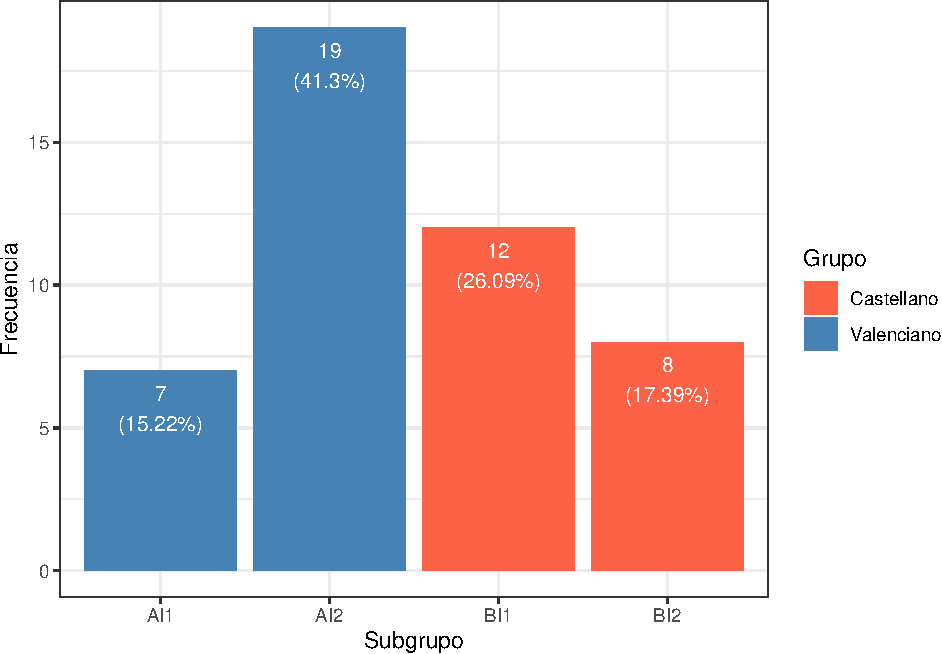
\includegraphics{informe_files/figure-latex/unnamed-chunk-3-1.pdf}

\hypertarget{uxedtems-2-y-3-conocuxedas-la-existencia-de-y}{%
\section{\texorpdfstring{Ítems 2 y 3: ¿Conocías la existencia de
\texttt{R} y
\texttt{R Markdown}?}{Ítems 2 y 3: ¿Conocías la existencia de  y ?}}\label{uxedtems-2-y-3-conocuxedas-la-existencia-de-y}}

\begin{Shaded}
\begin{Highlighting}[]
\FunctionTok{summary}\NormalTok{(encuesta[, }\FunctionTok{c}\NormalTok{(}\StringTok{"P2"}\NormalTok{, }\StringTok{"P3"}\NormalTok{)])}
\end{Highlighting}
\end{Shaded}

\begin{verbatim}
##     P2        P3    
##  No  :40   No  :45  
##  Si  : 6   Si  : 0  
##  NA's: 1   NA's: 2
\end{verbatim}

\hypertarget{uxedtem-4-has-sentido-frustraciuxf3n-mientras-aprenduxedas}{%
\section{\texorpdfstring{Ítem 4: ¿Has sentido frustración mientras
aprendías
\texttt{R Markdown}?}{Ítem 4: ¿Has sentido frustración mientras aprendías ?}}\label{uxedtem-4-has-sentido-frustraciuxf3n-mientras-aprenduxedas}}

\begin{Shaded}
\begin{Highlighting}[]
\NormalTok{df4 }\OtherTok{\textless{}{-}} \FunctionTok{data.frame}\NormalTok{(}\AttributeTok{subgrupo =} \FunctionTok{rep}\NormalTok{(}\FunctionTok{levels}\NormalTok{(encuesta}\SpecialCharTok{$}\NormalTok{P1), }\AttributeTok{each =} \FunctionTok{length}\NormalTok{(}\FunctionTok{levels}\NormalTok{(encuesta}\SpecialCharTok{$}\NormalTok{P4))),}
                  \AttributeTok{respuesta =} \FunctionTok{rep}\NormalTok{(}\FunctionTok{levels}\NormalTok{(encuesta}\SpecialCharTok{$}\NormalTok{P4), }\AttributeTok{times =} \FunctionTok{length}\NormalTok{(}\FunctionTok{levels}\NormalTok{(encuesta}\SpecialCharTok{$}\NormalTok{P1))),}
                  \AttributeTok{frecuencia =} \FunctionTok{as.numeric}\NormalTok{(}\FunctionTok{unlist}\NormalTok{(}\FunctionTok{by}\NormalTok{(encuesta}\SpecialCharTok{$}\NormalTok{P4, encuesta}\SpecialCharTok{$}\NormalTok{P1, table))))}
\NormalTok{df4}\SpecialCharTok{$}\NormalTok{porcentaje }\OtherTok{\textless{}{-}} \FunctionTok{paste0}\NormalTok{(}\StringTok{"("}\NormalTok{, }\FunctionTok{round}\NormalTok{(}\FunctionTok{as.numeric}\NormalTok{(}\FunctionTok{unlist}\NormalTok{(}\FunctionTok{by}\NormalTok{(encuesta}\SpecialCharTok{$}\NormalTok{P4, encuesta}\SpecialCharTok{$}\NormalTok{P1, }\ControlFlowTok{function}\NormalTok{(x) \{}\FunctionTok{table}\NormalTok{(x)}\SpecialCharTok{/}\FunctionTok{sum}\NormalTok{(}\FunctionTok{table}\NormalTok{(x))\}))) }\SpecialCharTok{*} \DecValTok{100}\NormalTok{, }\DecValTok{2}\NormalTok{), }\StringTok{"\%"}\NormalTok{, }\StringTok{")"}\NormalTok{)}
\NormalTok{df4}
\end{Highlighting}
\end{Shaded}

\begin{verbatim}
##   subgrupo respuesta frecuencia porcentaje
## 1      BI1        No          2   (16.67%)
## 2      BI1        Si         10   (83.33%)
## 3      BI2        No          3    (37.5%)
## 4      BI2        Si          5    (62.5%)
## 5      AI1        No          2   (28.57%)
## 6      AI1        Si          5   (71.43%)
## 7      AI2        No          3   (15.79%)
## 8      AI2        Si         16   (84.21%)
\end{verbatim}

\begin{Shaded}
\begin{Highlighting}[]
\NormalTok{p }\OtherTok{\textless{}{-}} \FunctionTok{ggplot}\NormalTok{(}\AttributeTok{data =}\NormalTok{ df4, }\FunctionTok{aes}\NormalTok{(}\AttributeTok{x =}\NormalTok{ subgrupo, }\AttributeTok{y =}\NormalTok{ frecuencia, }\AttributeTok{fill =}\NormalTok{ respuesta)) }\SpecialCharTok{+} 
  \FunctionTok{geom\_bar}\NormalTok{(}\AttributeTok{stat =} \StringTok{"identity"}\NormalTok{, }\AttributeTok{position=}\FunctionTok{position\_dodge}\NormalTok{()) }\SpecialCharTok{+}
  \FunctionTok{theme\_bw}\NormalTok{() }\SpecialCharTok{+} \FunctionTok{labs}\NormalTok{(}\AttributeTok{x =} \StringTok{"Subgrupo"}\NormalTok{, }\AttributeTok{y =} \StringTok{"Frecuencia"}\NormalTok{, }\AttributeTok{fill =} \StringTok{"Respuesta"}\NormalTok{) }\SpecialCharTok{+}
  \FunctionTok{geom\_text}\NormalTok{(}\FunctionTok{aes}\NormalTok{(}\AttributeTok{label =}\NormalTok{ frecuencia), }\AttributeTok{vjust =} \FloatTok{1.75}\NormalTok{, }\AttributeTok{position =} \FunctionTok{position\_dodge}\NormalTok{(}\FloatTok{0.9}\NormalTok{), }
            \AttributeTok{color =} \StringTok{"white"}\NormalTok{, }\AttributeTok{size =} \FloatTok{2.75}\NormalTok{) }\SpecialCharTok{+}
  \FunctionTok{geom\_text}\NormalTok{(}\FunctionTok{aes}\NormalTok{(}\AttributeTok{label =}\NormalTok{ porcentaje), }\AttributeTok{vjust =} \FloatTok{3.5}\NormalTok{, }\AttributeTok{position =} \FunctionTok{position\_dodge}\NormalTok{(}\FloatTok{0.9}\NormalTok{), }
            \AttributeTok{color =} \StringTok{"white"}\NormalTok{, }\AttributeTok{size =} \FloatTok{2.75}\NormalTok{) }\SpecialCharTok{+}
  \FunctionTok{scale\_fill\_manual}\NormalTok{(}\AttributeTok{values =} \FunctionTok{c}\NormalTok{(}\StringTok{"No"} \OtherTok{=} \StringTok{"forestgreen"}\NormalTok{, }\StringTok{"Si"} \OtherTok{=} \StringTok{"firebrick"}\NormalTok{))}
\NormalTok{p}
\end{Highlighting}
\end{Shaded}

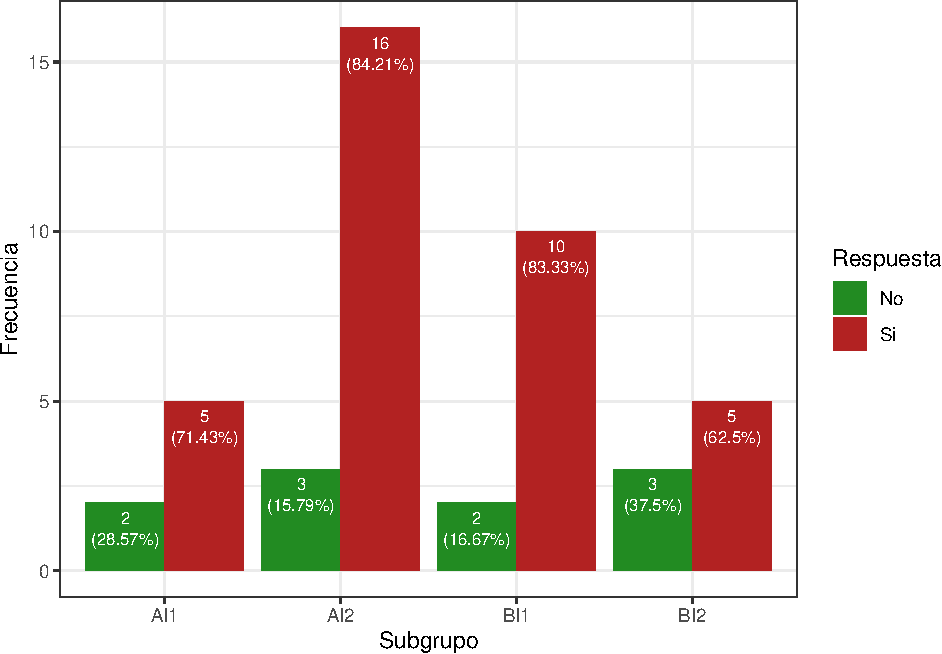
\includegraphics{informe_files/figure-latex/unnamed-chunk-5-1.pdf}

\hypertarget{uxedtem-5-en-caso-afirmativo-esa-frustraciuxf3n-ha-terminado-por-desaparecer}{%
\section{Ítem 5: En caso afirmativo, ¿esa frustración ha terminado por
desaparecer?}\label{uxedtem-5-en-caso-afirmativo-esa-frustraciuxf3n-ha-terminado-por-desaparecer}}

\begin{Shaded}
\begin{Highlighting}[]
\NormalTok{df5 }\OtherTok{\textless{}{-}} \FunctionTok{data.frame}\NormalTok{(}\AttributeTok{subgrupo =} \FunctionTok{rep}\NormalTok{(}\FunctionTok{levels}\NormalTok{(encuesta}\SpecialCharTok{$}\NormalTok{P1), }\AttributeTok{each =} \FunctionTok{length}\NormalTok{(}\FunctionTok{levels}\NormalTok{(encuesta}\SpecialCharTok{$}\NormalTok{P5))),}
                  \AttributeTok{respuesta =} \FunctionTok{rep}\NormalTok{(}\FunctionTok{levels}\NormalTok{(encuesta}\SpecialCharTok{$}\NormalTok{P5), }\AttributeTok{times =} \FunctionTok{length}\NormalTok{(}\FunctionTok{levels}\NormalTok{(encuesta}\SpecialCharTok{$}\NormalTok{P1))),}
                  \AttributeTok{frecuencia =} \FunctionTok{as.numeric}\NormalTok{(}\FunctionTok{unlist}\NormalTok{(}\FunctionTok{by}\NormalTok{(encuesta}\SpecialCharTok{$}\NormalTok{P5[}\FunctionTok{which}\NormalTok{(encuesta}\SpecialCharTok{$}\NormalTok{P4 }\SpecialCharTok{==} \StringTok{"Si"}\NormalTok{)], encuesta}\SpecialCharTok{$}\NormalTok{P1[}\FunctionTok{which}\NormalTok{(encuesta}\SpecialCharTok{$}\NormalTok{P4 }\SpecialCharTok{==} \StringTok{"Si"}\NormalTok{)], table))))}
\NormalTok{df5}\SpecialCharTok{$}\NormalTok{porcentaje }\OtherTok{\textless{}{-}} \FunctionTok{paste0}\NormalTok{(}\StringTok{"("}\NormalTok{, }\FunctionTok{round}\NormalTok{(}\FunctionTok{as.numeric}\NormalTok{(}\FunctionTok{unlist}\NormalTok{(}\FunctionTok{by}\NormalTok{(encuesta}\SpecialCharTok{$}\NormalTok{P5[}\FunctionTok{which}\NormalTok{(encuesta}\SpecialCharTok{$}\NormalTok{P4 }\SpecialCharTok{==} \StringTok{"Si"}\NormalTok{)], encuesta}\SpecialCharTok{$}\NormalTok{P1[}\FunctionTok{which}\NormalTok{(encuesta}\SpecialCharTok{$}\NormalTok{P4 }\SpecialCharTok{==} \StringTok{"Si"}\NormalTok{)], }\ControlFlowTok{function}\NormalTok{(x) \{}\FunctionTok{table}\NormalTok{(x)}\SpecialCharTok{/}\FunctionTok{sum}\NormalTok{(}\FunctionTok{table}\NormalTok{(x))\}))) }\SpecialCharTok{*} \DecValTok{100}\NormalTok{, }\DecValTok{2}\NormalTok{), }\StringTok{"\%"}\NormalTok{, }\StringTok{")"}\NormalTok{)}
\NormalTok{df5}
\end{Highlighting}
\end{Shaded}

\begin{verbatim}
##   subgrupo respuesta frecuencia porcentaje
## 1      BI1        No          2      (20%)
## 2      BI1        Si          8      (80%)
## 3      BI2        No          0       (0%)
## 4      BI2        Si          5     (100%)
## 5      AI1        No          0       (0%)
## 6      AI1        Si          5     (100%)
## 7      AI2        No          9      (60%)
## 8      AI2        Si          6      (40%)
\end{verbatim}

\begin{Shaded}
\begin{Highlighting}[]
\NormalTok{p }\OtherTok{\textless{}{-}} \FunctionTok{ggplot}\NormalTok{(}\AttributeTok{data =}\NormalTok{ df5, }\FunctionTok{aes}\NormalTok{(}\AttributeTok{x =}\NormalTok{ subgrupo, }\AttributeTok{y =}\NormalTok{ frecuencia, }\AttributeTok{fill =}\NormalTok{ respuesta)) }\SpecialCharTok{+} 
  \FunctionTok{geom\_bar}\NormalTok{(}\AttributeTok{stat =} \StringTok{"identity"}\NormalTok{, }\AttributeTok{position=}\FunctionTok{position\_dodge}\NormalTok{()) }\SpecialCharTok{+}
  \FunctionTok{theme\_bw}\NormalTok{() }\SpecialCharTok{+} \FunctionTok{labs}\NormalTok{(}\AttributeTok{x =} \StringTok{"Subgrupo"}\NormalTok{, }\AttributeTok{y =} \StringTok{"Frecuencia"}\NormalTok{, }\AttributeTok{fill =} \StringTok{"Respuesta"}\NormalTok{) }\SpecialCharTok{+}
  \FunctionTok{geom\_text}\NormalTok{(}\FunctionTok{aes}\NormalTok{(}\AttributeTok{label =}\NormalTok{ frecuencia), }\AttributeTok{vjust =} \FloatTok{1.75}\NormalTok{, }\AttributeTok{position =} \FunctionTok{position\_dodge}\NormalTok{(}\FloatTok{0.9}\NormalTok{), }
            \AttributeTok{color =} \StringTok{"white"}\NormalTok{, }\AttributeTok{size =} \FloatTok{2.75}\NormalTok{) }\SpecialCharTok{+}
  \FunctionTok{geom\_text}\NormalTok{(}\FunctionTok{aes}\NormalTok{(}\AttributeTok{label =}\NormalTok{ porcentaje), }\AttributeTok{vjust =} \FloatTok{3.5}\NormalTok{, }\AttributeTok{position =} \FunctionTok{position\_dodge}\NormalTok{(}\FloatTok{0.9}\NormalTok{), }
            \AttributeTok{color =} \StringTok{"white"}\NormalTok{, }\AttributeTok{size =} \FloatTok{2.75}\NormalTok{) }\SpecialCharTok{+}
  \FunctionTok{scale\_fill\_manual}\NormalTok{(}\AttributeTok{values =} \FunctionTok{c}\NormalTok{(}\StringTok{"No"} \OtherTok{=} \StringTok{"firebrick"}\NormalTok{, }\StringTok{"Si"} \OtherTok{=} \StringTok{"forestgreen"}\NormalTok{)) }\SpecialCharTok{+}
  \FunctionTok{scale\_y\_continuous}\NormalTok{(}\AttributeTok{breaks =} \FunctionTok{seq}\NormalTok{(}\DecValTok{0}\NormalTok{, }\DecValTok{10}\NormalTok{, }\AttributeTok{by =} \DecValTok{2}\NormalTok{))}
\NormalTok{p}
\end{Highlighting}
\end{Shaded}

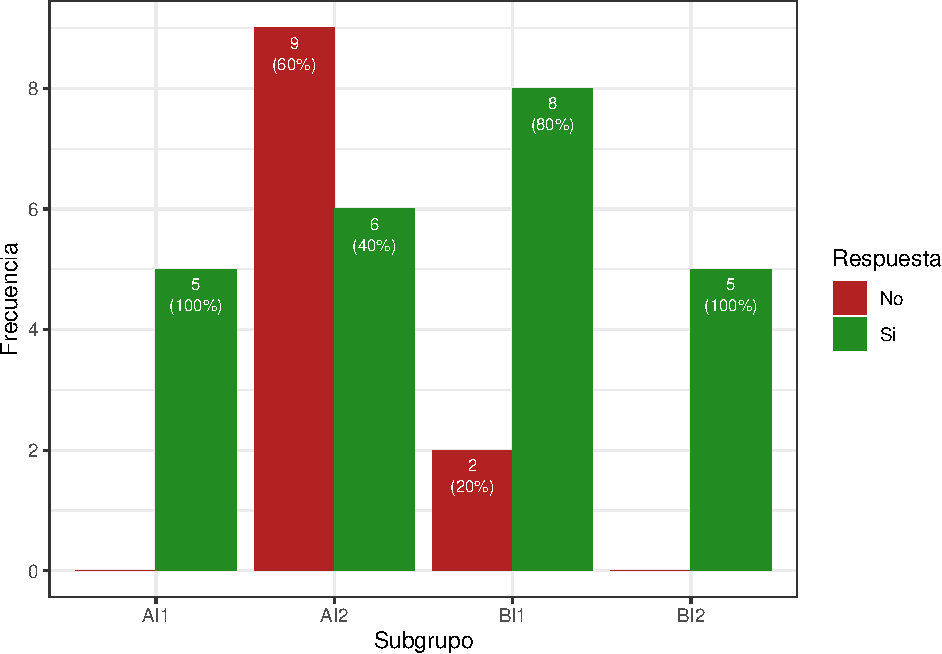
\includegraphics{informe_files/figure-latex/unnamed-chunk-6-1.pdf}

\hypertarget{uxedtem-6-consideras-que-te-ha-facilitado-la-entrega-de-tareas}{%
\section{\texorpdfstring{Ítem 6: ¿Consideras que \texttt{R Markdown} te
ha facilitado la entrega de
tareas?}{Ítem 6: ¿Consideras que  te ha facilitado la entrega de tareas?}}\label{uxedtem-6-consideras-que-te-ha-facilitado-la-entrega-de-tareas}}

\begin{Shaded}
\begin{Highlighting}[]
\NormalTok{df6 }\OtherTok{\textless{}{-}} \FunctionTok{data.frame}\NormalTok{(}\AttributeTok{subgrupo =} \FunctionTok{rep}\NormalTok{(}\FunctionTok{levels}\NormalTok{(encuesta}\SpecialCharTok{$}\NormalTok{P1), }\AttributeTok{each =} \FunctionTok{length}\NormalTok{(}\FunctionTok{levels}\NormalTok{(encuesta}\SpecialCharTok{$}\NormalTok{P6))),}
                  \AttributeTok{respuesta =} \FunctionTok{rep}\NormalTok{(}\FunctionTok{levels}\NormalTok{(encuesta}\SpecialCharTok{$}\NormalTok{P6), }\AttributeTok{times =} \FunctionTok{length}\NormalTok{(}\FunctionTok{levels}\NormalTok{(encuesta}\SpecialCharTok{$}\NormalTok{P1))),}
                  \AttributeTok{frecuencia =} \FunctionTok{as.numeric}\NormalTok{(}\FunctionTok{unlist}\NormalTok{(}\FunctionTok{by}\NormalTok{(encuesta}\SpecialCharTok{$}\NormalTok{P6, encuesta}\SpecialCharTok{$}\NormalTok{P1, table))))}
\NormalTok{df6}\SpecialCharTok{$}\NormalTok{porcentaje }\OtherTok{\textless{}{-}} \FunctionTok{paste0}\NormalTok{(}\StringTok{"("}\NormalTok{, }\FunctionTok{round}\NormalTok{(}\FunctionTok{as.numeric}\NormalTok{(}\FunctionTok{unlist}\NormalTok{(}\FunctionTok{by}\NormalTok{(encuesta}\SpecialCharTok{$}\NormalTok{P6, encuesta}\SpecialCharTok{$}\NormalTok{P1, }\ControlFlowTok{function}\NormalTok{(x) \{}\FunctionTok{table}\NormalTok{(x)}\SpecialCharTok{/}\FunctionTok{sum}\NormalTok{(}\FunctionTok{table}\NormalTok{(x))\}))) }\SpecialCharTok{*} \DecValTok{100}\NormalTok{, }\DecValTok{2}\NormalTok{), }\StringTok{"\%"}\NormalTok{, }\StringTok{")"}\NormalTok{)}
\NormalTok{df6}
\end{Highlighting}
\end{Shaded}

\begin{verbatim}
##   subgrupo respuesta frecuencia porcentaje
## 1      BI1        No          1    (8.33%)
## 2      BI1        Si         11   (91.67%)
## 3      BI2        No          0       (0%)
## 4      BI2        Si          8     (100%)
## 5      AI1        No          1   (14.29%)
## 6      AI1        Si          6   (85.71%)
## 7      AI2        No          2   (11.76%)
## 8      AI2        Si         15   (88.24%)
\end{verbatim}

\begin{Shaded}
\begin{Highlighting}[]
\NormalTok{p }\OtherTok{\textless{}{-}} \FunctionTok{ggplot}\NormalTok{(}\AttributeTok{data =}\NormalTok{ df6, }\FunctionTok{aes}\NormalTok{(}\AttributeTok{x =}\NormalTok{ subgrupo, }\AttributeTok{y =}\NormalTok{ frecuencia, }\AttributeTok{fill =}\NormalTok{ respuesta)) }\SpecialCharTok{+} 
  \FunctionTok{geom\_bar}\NormalTok{(}\AttributeTok{stat =} \StringTok{"identity"}\NormalTok{, }\AttributeTok{position=}\FunctionTok{position\_dodge}\NormalTok{()) }\SpecialCharTok{+}
  \FunctionTok{theme\_bw}\NormalTok{() }\SpecialCharTok{+} \FunctionTok{labs}\NormalTok{(}\AttributeTok{x =} \StringTok{"Subgrupo"}\NormalTok{, }\AttributeTok{y =} \StringTok{"Frecuencia"}\NormalTok{, }\AttributeTok{fill =} \StringTok{"Respuesta"}\NormalTok{) }\SpecialCharTok{+}
  \FunctionTok{geom\_text}\NormalTok{(}\FunctionTok{aes}\NormalTok{(}\AttributeTok{label =}\NormalTok{ frecuencia), }\AttributeTok{vjust =} \FloatTok{1.75}\NormalTok{, }\AttributeTok{position =} \FunctionTok{position\_dodge}\NormalTok{(}\FloatTok{0.9}\NormalTok{), }
            \AttributeTok{color =} \StringTok{"white"}\NormalTok{, }\AttributeTok{size =} \FloatTok{1.75}\NormalTok{) }\SpecialCharTok{+}
  \FunctionTok{geom\_text}\NormalTok{(}\FunctionTok{aes}\NormalTok{(}\AttributeTok{label =}\NormalTok{ porcentaje), }\AttributeTok{vjust =} \FloatTok{3.5}\NormalTok{, }\AttributeTok{position =} \FunctionTok{position\_dodge}\NormalTok{(}\FloatTok{0.9}\NormalTok{), }
            \AttributeTok{color =} \StringTok{"white"}\NormalTok{, }\AttributeTok{size =} \FloatTok{1.75}\NormalTok{) }\SpecialCharTok{+}
  \FunctionTok{scale\_fill\_manual}\NormalTok{(}\AttributeTok{values =} \FunctionTok{c}\NormalTok{(}\StringTok{"No"} \OtherTok{=} \StringTok{"firebrick"}\NormalTok{, }\StringTok{"Si"} \OtherTok{=} \StringTok{"forestgreen"}\NormalTok{))}
\NormalTok{p}
\end{Highlighting}
\end{Shaded}

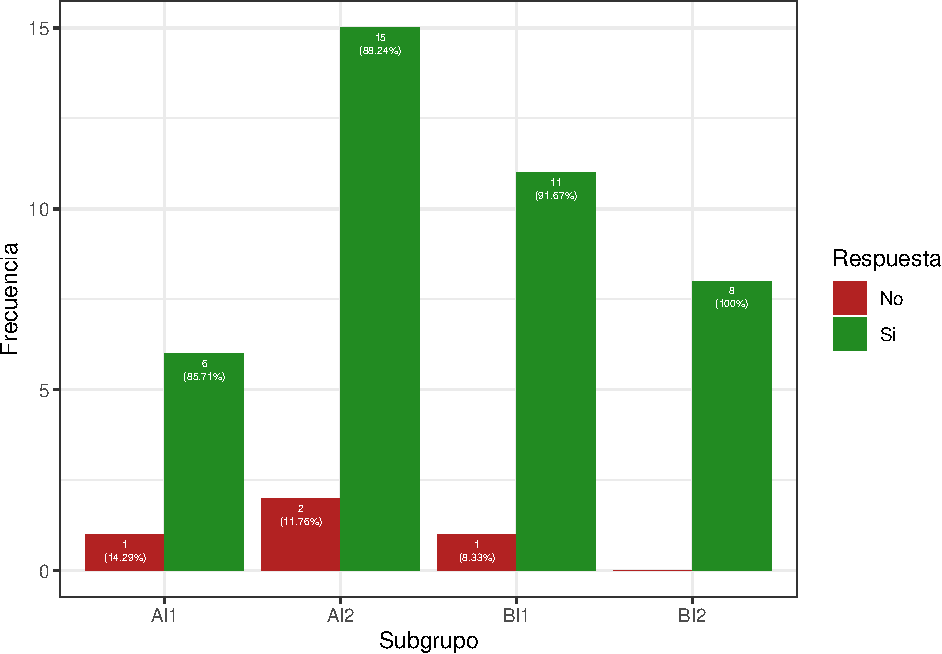
\includegraphics{informe_files/figure-latex/unnamed-chunk-7-1.pdf}

\hypertarget{uxedtem-7-cuxf3mo-calificaruxedas-la-dificultad-de-aprender}{%
\section{\texorpdfstring{Ítem 7: ¿Cómo calificarías la dificultad de
aprender
\texttt{R Markdown}?}{Ítem 7: ¿Cómo calificarías la dificultad de aprender ?}}\label{uxedtem-7-cuxf3mo-calificaruxedas-la-dificultad-de-aprender}}

\begin{Shaded}
\begin{Highlighting}[]
\NormalTok{df7 }\OtherTok{\textless{}{-}} \FunctionTok{data.frame}\NormalTok{(}\AttributeTok{grupo =} \FunctionTok{as.character}\NormalTok{(encuesta}\SpecialCharTok{$}\NormalTok{P0),}
                  \AttributeTok{subgrupo =} \FunctionTok{as.character}\NormalTok{(encuesta}\SpecialCharTok{$}\NormalTok{P1),}
                  \AttributeTok{respuesta =} \FunctionTok{as.numeric}\NormalTok{(encuesta}\SpecialCharTok{$}\NormalTok{P7))}
\NormalTok{df7}
\end{Highlighting}
\end{Shaded}

\begin{verbatim}
##         grupo subgrupo respuesta
## 1  Castellano      BI1         2
## 2  Castellano      BI1         3
## 3  Castellano      BI1         3
## 4  Castellano      BI1         4
## 5  Castellano      BI2         2
## 6  Castellano      BI1         3
## 7  Castellano      BI1         3
## 8  Castellano      BI1         2
## 9  Castellano      BI1         4
## 10 Castellano      BI1         3
## 11 Castellano      BI2         4
## 12 Castellano      BI1         2
## 13 Castellano      BI1         4
## 14 Castellano      BI2         1
## 15 Castellano      BI2         2
## 16 Castellano      BI1         3
## 17 Castellano      BI2         3
## 18 Castellano      BI2         1
## 19 Castellano      BI2         4
## 20 Castellano      BI2         3
## 21 Valenciano      AI1         1
## 22 Valenciano      AI1         3
## 23 Valenciano      AI2         3
## 24 Valenciano      AI1         3
## 25 Valenciano      AI2         3
## 26 Valenciano      AI2         4
## 27 Valenciano      AI2         5
## 28 Valenciano      AI2         3
## 29 Valenciano      AI1         3
## 30 Valenciano      AI2         4
## 31 Valenciano      AI2         2
## 32 Valenciano      AI2         4
## 33 Valenciano      AI2         3
## 34 Valenciano      AI2         3
## 35 Valenciano      AI2         4
## 36 Valenciano      AI2         3
## 37 Valenciano      AI2         5
## 38 Valenciano     <NA>         3
## 39 Valenciano      AI2         4
## 40 Valenciano      AI1         4
## 41 Valenciano      AI2         3
## 42 Valenciano      AI1         3
## 43 Valenciano      AI2         3
## 44 Valenciano      AI2         5
## 45 Valenciano      AI2         2
## 46 Valenciano      AI1         3
## 47 Valenciano      AI2         3
\end{verbatim}

\begin{Shaded}
\begin{Highlighting}[]
\NormalTok{p }\OtherTok{\textless{}{-}} \FunctionTok{ggplot}\NormalTok{(}\AttributeTok{data =} \FunctionTok{subset}\NormalTok{(df7, }\SpecialCharTok{!}\FunctionTok{is.na}\NormalTok{(subgrupo)), }\FunctionTok{aes}\NormalTok{(}\AttributeTok{x =}\NormalTok{ subgrupo, }\AttributeTok{y =}\NormalTok{ respuesta)) }\SpecialCharTok{+} 
  \FunctionTok{geom\_dotplot}\NormalTok{(}\FunctionTok{aes}\NormalTok{(}\AttributeTok{fill =}\NormalTok{ grupo), }\AttributeTok{binaxis =} \StringTok{"y"}\NormalTok{, }\AttributeTok{stackdir =} \StringTok{"center"}\NormalTok{, }\AttributeTok{dotsize =} \FloatTok{0.75}\NormalTok{) }\SpecialCharTok{+}
  \FunctionTok{theme\_bw}\NormalTok{() }\SpecialCharTok{+} \FunctionTok{labs}\NormalTok{(}\AttributeTok{x =} \StringTok{"Subgrupo"}\NormalTok{, }\AttributeTok{y =} \StringTok{"Respuesta"}\NormalTok{, }\AttributeTok{fill =} \StringTok{"Grupo"}\NormalTok{) }\SpecialCharTok{+}
  \FunctionTok{scale\_fill\_manual}\NormalTok{(}\AttributeTok{values =} \FunctionTok{c}\NormalTok{(}\StringTok{"Castellano"} \OtherTok{=} \StringTok{"tomato"}\NormalTok{, }\StringTok{"Valenciano"} \OtherTok{=} \StringTok{"steelblue"}\NormalTok{)) }\SpecialCharTok{+} 
  \FunctionTok{stat\_summary}\NormalTok{(}\AttributeTok{fun =}\NormalTok{ mean, }\AttributeTok{geom =} \StringTok{"point"}\NormalTok{, }\AttributeTok{shape =} \DecValTok{18}\NormalTok{, }\AttributeTok{size =} \DecValTok{3}\NormalTok{, }\AttributeTok{color =} \StringTok{"black"}\NormalTok{) }\SpecialCharTok{+}
  \FunctionTok{scale\_y\_continuous}\NormalTok{(}\AttributeTok{breaks =} \DecValTok{1}\SpecialCharTok{:}\FunctionTok{length}\NormalTok{(}\FunctionTok{levels}\NormalTok{(encuesta}\SpecialCharTok{$}\NormalTok{P7)),}
                     \AttributeTok{labels =} \FunctionTok{c}\NormalTok{(}\StringTok{"Muy facil (1)"}\NormalTok{, }\StringTok{"Facil (2)"}\NormalTok{, }\StringTok{"Normal (3)"}\NormalTok{, }\StringTok{"Dificil (4)"}\NormalTok{, }\StringTok{"Muy dificil (5)"}\NormalTok{))}
\NormalTok{p}
\end{Highlighting}
\end{Shaded}

\begin{verbatim}
## Bin width defaults to 1/30 of the range of the data. Pick better value with
## `binwidth`.
\end{verbatim}

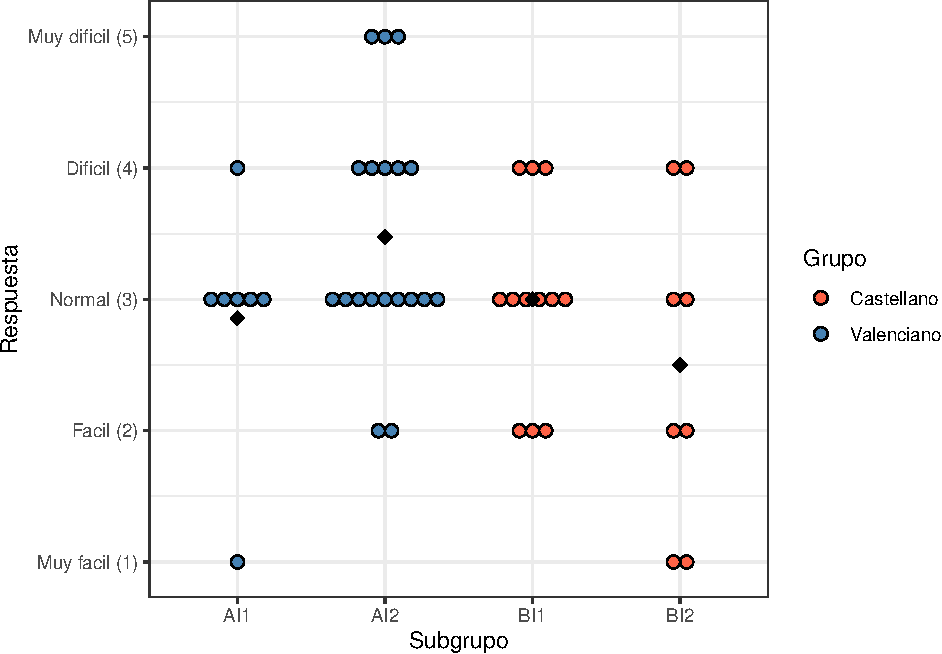
\includegraphics{informe_files/figure-latex/unnamed-chunk-8-1.pdf}

\hypertarget{uxedtem-8-te-ha-facilitado-comprender-los-anuxe1lisis-estaduxedsticos}{%
\section{\texorpdfstring{Ítem 8: ¿\texttt{R Markdown} te ha facilitado
comprender los análisis
estadísticos?}{Ítem 8: ¿ te ha facilitado comprender los análisis estadísticos?}}\label{uxedtem-8-te-ha-facilitado-comprender-los-anuxe1lisis-estaduxedsticos}}

\begin{Shaded}
\begin{Highlighting}[]
\NormalTok{df8 }\OtherTok{\textless{}{-}} \FunctionTok{data.frame}\NormalTok{(}\AttributeTok{grupo =} \FunctionTok{as.character}\NormalTok{(encuesta}\SpecialCharTok{$}\NormalTok{P0),}
                  \AttributeTok{subgrupo =} \FunctionTok{as.character}\NormalTok{(encuesta}\SpecialCharTok{$}\NormalTok{P1),}
                  \AttributeTok{respuesta =} \FunctionTok{as.numeric}\NormalTok{(encuesta}\SpecialCharTok{$}\NormalTok{P8))}
\NormalTok{df8}
\end{Highlighting}
\end{Shaded}

\begin{verbatim}
##         grupo subgrupo respuesta
## 1  Castellano      BI1         2
## 2  Castellano      BI1         3
## 3  Castellano      BI1         3
## 4  Castellano      BI1         5
## 5  Castellano      BI2         2
## 6  Castellano      BI1         2
## 7  Castellano      BI1         2
## 8  Castellano      BI1         2
## 9  Castellano      BI1         3
## 10 Castellano      BI1         2
## 11 Castellano      BI2         4
## 12 Castellano      BI1         2
## 13 Castellano      BI1         1
## 14 Castellano      BI2         1
## 15 Castellano      BI2         1
## 16 Castellano      BI1         5
## 17 Castellano      BI2         1
## 18 Castellano      BI2         1
## 19 Castellano      BI2         1
## 20 Castellano      BI2         2
## 21 Valenciano      AI1         2
## 22 Valenciano      AI1         2
## 23 Valenciano      AI2         2
## 24 Valenciano      AI1         1
## 25 Valenciano      AI2         4
## 26 Valenciano      AI2         3
## 27 Valenciano      AI2         5
## 28 Valenciano      AI2         2
## 29 Valenciano      AI1         3
## 30 Valenciano      AI2         4
## 31 Valenciano      AI2         2
## 32 Valenciano      AI2         4
## 33 Valenciano      AI2         3
## 34 Valenciano      AI2         3
## 35 Valenciano      AI2         3
## 36 Valenciano      AI2         4
## 37 Valenciano      AI2         3
## 38 Valenciano     <NA>         3
## 39 Valenciano      AI2        NA
## 40 Valenciano      AI1         3
## 41 Valenciano      AI2        NA
## 42 Valenciano      AI1         2
## 43 Valenciano      AI2         2
## 44 Valenciano      AI2        NA
## 45 Valenciano      AI2         4
## 46 Valenciano      AI1         3
## 47 Valenciano      AI2         2
\end{verbatim}

\begin{Shaded}
\begin{Highlighting}[]
\NormalTok{p }\OtherTok{\textless{}{-}} \FunctionTok{ggplot}\NormalTok{(}\AttributeTok{data =} \FunctionTok{subset}\NormalTok{(df8, }\SpecialCharTok{!}\FunctionTok{is.na}\NormalTok{(subgrupo)), }\FunctionTok{aes}\NormalTok{(}\AttributeTok{x =}\NormalTok{ subgrupo, }\AttributeTok{y =}\NormalTok{ respuesta)) }\SpecialCharTok{+} 
  \FunctionTok{geom\_dotplot}\NormalTok{(}\FunctionTok{aes}\NormalTok{(}\AttributeTok{fill =}\NormalTok{ grupo), }\AttributeTok{binaxis =} \StringTok{"y"}\NormalTok{, }\AttributeTok{stackdir =} \StringTok{"center"}\NormalTok{, }\AttributeTok{dotsize =} \FloatTok{0.75}\NormalTok{) }\SpecialCharTok{+}
  \FunctionTok{theme\_bw}\NormalTok{() }\SpecialCharTok{+} \FunctionTok{labs}\NormalTok{(}\AttributeTok{x =} \StringTok{"Subgrupo"}\NormalTok{, }\AttributeTok{y =} \StringTok{"Respuesta"}\NormalTok{, }\AttributeTok{fill =} \StringTok{"Grupo"}\NormalTok{) }\SpecialCharTok{+}
  \FunctionTok{scale\_fill\_manual}\NormalTok{(}\AttributeTok{values =} \FunctionTok{c}\NormalTok{(}\StringTok{"Castellano"} \OtherTok{=} \StringTok{"tomato"}\NormalTok{, }\StringTok{"Valenciano"} \OtherTok{=} \StringTok{"steelblue"}\NormalTok{)) }\SpecialCharTok{+} 
  \FunctionTok{stat\_summary}\NormalTok{(}\AttributeTok{fun =}\NormalTok{ mean, }\AttributeTok{geom =} \StringTok{"point"}\NormalTok{, }\AttributeTok{shape =} \DecValTok{18}\NormalTok{, }\AttributeTok{size =} \DecValTok{3}\NormalTok{, }\AttributeTok{color =} \StringTok{"black"}\NormalTok{) }\SpecialCharTok{+}
  \FunctionTok{scale\_y\_continuous}\NormalTok{(}\AttributeTok{breaks =} \DecValTok{1}\SpecialCharTok{:}\FunctionTok{length}\NormalTok{(}\FunctionTok{levels}\NormalTok{(encuesta}\SpecialCharTok{$}\NormalTok{P7)),}
                     \AttributeTok{labels =} \FunctionTok{c}\NormalTok{(}\StringTok{"Facil. mucho (1)"}\NormalTok{, }\StringTok{"Facilitado (2)"}\NormalTok{, }\StringTok{"Normal (3)"}\NormalTok{, }\StringTok{"Dificultado (4)"}\NormalTok{, }\StringTok{"Dific. mucho (5)"}\NormalTok{))}
\NormalTok{p}
\end{Highlighting}
\end{Shaded}

\begin{verbatim}
## Bin width defaults to 1/30 of the range of the data. Pick better value with
## `binwidth`.
\end{verbatim}

\begin{verbatim}
## Warning: Removed 3 rows containing missing values or values outside the scale range
## (`stat_bindot()`).
\end{verbatim}

\begin{verbatim}
## Warning: Removed 3 rows containing non-finite outside the scale range
## (`stat_summary()`).
\end{verbatim}

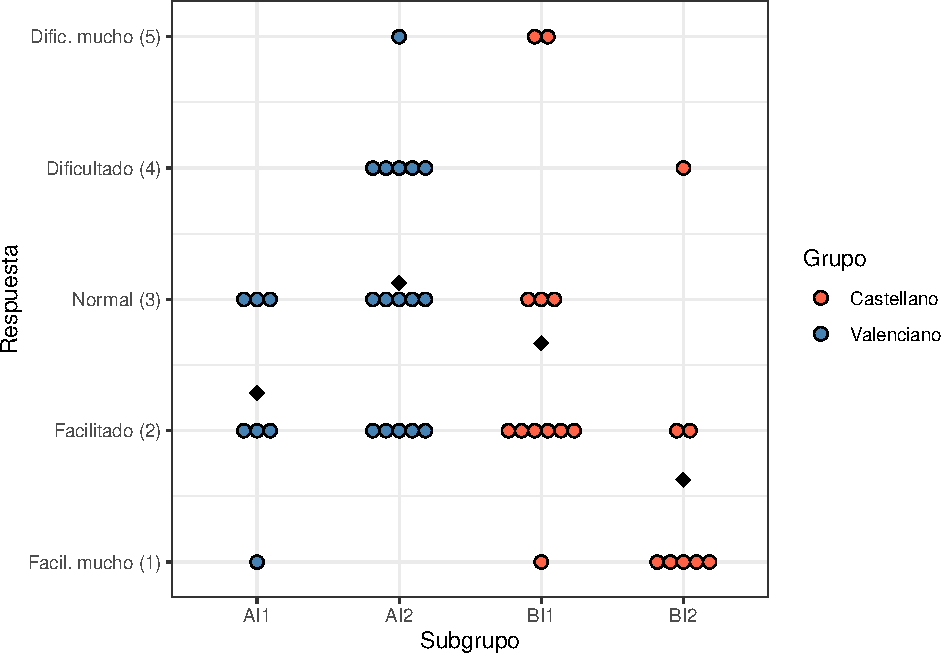
\includegraphics{informe_files/figure-latex/unnamed-chunk-9-1.pdf}

\hypertarget{uxedtem-9-cuuxe1l-ha-sido-tu-grado-de-satisfacciuxf3n-utilizando}{%
\section{\texorpdfstring{Ítem 9: ¿Cuál ha sido tu grado de satisfacción
utilizando
\texttt{R Markdown}?}{Ítem 9: ¿Cuál ha sido tu grado de satisfacción utilizando ?}}\label{uxedtem-9-cuuxe1l-ha-sido-tu-grado-de-satisfacciuxf3n-utilizando}}

\begin{Shaded}
\begin{Highlighting}[]
\NormalTok{df9 }\OtherTok{\textless{}{-}} \FunctionTok{data.frame}\NormalTok{(}\AttributeTok{grupo =} \FunctionTok{as.character}\NormalTok{(encuesta}\SpecialCharTok{$}\NormalTok{P0),}
                  \AttributeTok{subgrupo =} \FunctionTok{as.character}\NormalTok{(encuesta}\SpecialCharTok{$}\NormalTok{P1),}
                  \AttributeTok{respuesta =} \FunctionTok{as.numeric}\NormalTok{(encuesta}\SpecialCharTok{$}\NormalTok{P9))}
\NormalTok{df9}
\end{Highlighting}
\end{Shaded}

\begin{verbatim}
##         grupo subgrupo respuesta
## 1  Castellano      BI1         1
## 2  Castellano      BI1         3
## 3  Castellano      BI1         3
## 4  Castellano      BI1         3
## 5  Castellano      BI2         2
## 6  Castellano      BI1         2
## 7  Castellano      BI1         2
## 8  Castellano      BI1        NA
## 9  Castellano      BI1         3
## 10 Castellano      BI1         2
## 11 Castellano      BI2         4
## 12 Castellano      BI1         2
## 13 Castellano      BI1         2
## 14 Castellano      BI2         1
## 15 Castellano      BI2         1
## 16 Castellano      BI1         5
## 17 Castellano      BI2         1
## 18 Castellano      BI2         1
## 19 Castellano      BI2         1
## 20 Castellano      BI2         3
## 21 Valenciano      AI1         1
## 22 Valenciano      AI1         2
## 23 Valenciano      AI2         2
## 24 Valenciano      AI1         2
## 25 Valenciano      AI2         4
## 26 Valenciano      AI2         3
## 27 Valenciano      AI2         4
## 28 Valenciano      AI2         2
## 29 Valenciano      AI1         3
## 30 Valenciano      AI2         5
## 31 Valenciano      AI2         2
## 32 Valenciano      AI2         4
## 33 Valenciano      AI2         3
## 34 Valenciano      AI2         3
## 35 Valenciano      AI2         2
## 36 Valenciano      AI2         4
## 37 Valenciano      AI2         3
## 38 Valenciano     <NA>         4
## 39 Valenciano      AI2         3
## 40 Valenciano      AI1         2
## 41 Valenciano      AI2        NA
## 42 Valenciano      AI1         2
## 43 Valenciano      AI2         3
## 44 Valenciano      AI2         4
## 45 Valenciano      AI2         2
## 46 Valenciano      AI1         4
## 47 Valenciano      AI2         2
\end{verbatim}

\begin{Shaded}
\begin{Highlighting}[]
\NormalTok{p }\OtherTok{\textless{}{-}} \FunctionTok{ggplot}\NormalTok{(}\AttributeTok{data =} \FunctionTok{subset}\NormalTok{(df9, }\SpecialCharTok{!}\FunctionTok{is.na}\NormalTok{(subgrupo)), }\FunctionTok{aes}\NormalTok{(}\AttributeTok{x =}\NormalTok{ subgrupo, }\AttributeTok{y =}\NormalTok{ respuesta)) }\SpecialCharTok{+} 
  \FunctionTok{geom\_dotplot}\NormalTok{(}\FunctionTok{aes}\NormalTok{(}\AttributeTok{fill =}\NormalTok{ grupo), }\AttributeTok{binaxis =} \StringTok{"y"}\NormalTok{, }\AttributeTok{stackdir =} \StringTok{"center"}\NormalTok{, }\AttributeTok{dotsize =} \FloatTok{0.75}\NormalTok{) }\SpecialCharTok{+}
  \FunctionTok{theme\_bw}\NormalTok{() }\SpecialCharTok{+} \FunctionTok{labs}\NormalTok{(}\AttributeTok{x =} \StringTok{"Subgrupo"}\NormalTok{, }\AttributeTok{y =} \StringTok{"Respuesta"}\NormalTok{, }\AttributeTok{fill =} \StringTok{"Grupo"}\NormalTok{) }\SpecialCharTok{+}
  \FunctionTok{scale\_fill\_manual}\NormalTok{(}\AttributeTok{values =} \FunctionTok{c}\NormalTok{(}\StringTok{"Castellano"} \OtherTok{=} \StringTok{"tomato"}\NormalTok{, }\StringTok{"Valenciano"} \OtherTok{=} \StringTok{"steelblue"}\NormalTok{)) }\SpecialCharTok{+} 
  \FunctionTok{stat\_summary}\NormalTok{(}\AttributeTok{fun =}\NormalTok{ mean, }\AttributeTok{geom =} \StringTok{"point"}\NormalTok{, }\AttributeTok{shape =} \DecValTok{18}\NormalTok{, }\AttributeTok{size =} \DecValTok{3}\NormalTok{, }\AttributeTok{color =} \StringTok{"black"}\NormalTok{) }\SpecialCharTok{+}
  \FunctionTok{scale\_y\_continuous}\NormalTok{(}\AttributeTok{breaks =} \DecValTok{1}\SpecialCharTok{:}\FunctionTok{length}\NormalTok{(}\FunctionTok{levels}\NormalTok{(encuesta}\SpecialCharTok{$}\NormalTok{P7)),}
                     \AttributeTok{labels =} \FunctionTok{c}\NormalTok{(}\StringTok{"Muy satisf. (1)"}\NormalTok{, }\StringTok{"Satisfecho (2)"}\NormalTok{, }\StringTok{"Normal (3)"}\NormalTok{, }\StringTok{"Insatisfecho (4)"}\NormalTok{, }\StringTok{"Muy insatisf. (5)"}\NormalTok{))}
\NormalTok{p}
\end{Highlighting}
\end{Shaded}

\begin{verbatim}
## Bin width defaults to 1/30 of the range of the data. Pick better value with
## `binwidth`.
\end{verbatim}

\begin{verbatim}
## Warning: Removed 2 rows containing missing values or values outside the scale range
## (`stat_bindot()`).
\end{verbatim}

\begin{verbatim}
## Warning: Removed 2 rows containing non-finite outside the scale range
## (`stat_summary()`).
\end{verbatim}

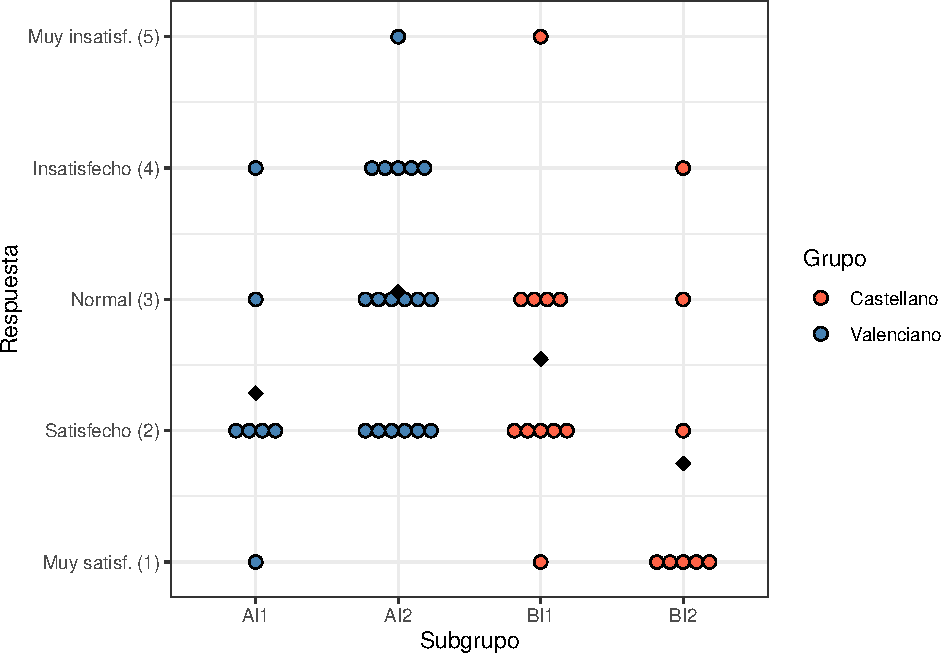
\includegraphics{informe_files/figure-latex/unnamed-chunk-10-1.pdf}

\hypertarget{uxedtem-10-consideras-que-es-una-herramienta-uxfatil}{%
\section{\texorpdfstring{Ítem 10: ¿Consideras que \texttt{R Markdown} es
una herramienta
útil?}{Ítem 10: ¿Consideras que  es una herramienta útil?}}\label{uxedtem-10-consideras-que-es-una-herramienta-uxfatil}}

\begin{Shaded}
\begin{Highlighting}[]
\NormalTok{df10 }\OtherTok{\textless{}{-}} \FunctionTok{data.frame}\NormalTok{(}\AttributeTok{subgrupo =} \FunctionTok{rep}\NormalTok{(}\FunctionTok{levels}\NormalTok{(encuesta}\SpecialCharTok{$}\NormalTok{P1), }\AttributeTok{each =} \FunctionTok{length}\NormalTok{(}\FunctionTok{levels}\NormalTok{(encuesta}\SpecialCharTok{$}\NormalTok{P10))),}
                   \AttributeTok{respuesta =} \FunctionTok{rep}\NormalTok{(}\FunctionTok{levels}\NormalTok{(encuesta}\SpecialCharTok{$}\NormalTok{P10), }\AttributeTok{times =} \FunctionTok{length}\NormalTok{(}\FunctionTok{levels}\NormalTok{(encuesta}\SpecialCharTok{$}\NormalTok{P1))),}
                   \AttributeTok{frecuencia =} \FunctionTok{as.numeric}\NormalTok{(}\FunctionTok{unlist}\NormalTok{(}\FunctionTok{by}\NormalTok{(encuesta}\SpecialCharTok{$}\NormalTok{P10, encuesta}\SpecialCharTok{$}\NormalTok{P1, table))))}
\NormalTok{df10}\SpecialCharTok{$}\NormalTok{porcentaje }\OtherTok{\textless{}{-}} \FunctionTok{paste0}\NormalTok{(}\StringTok{"("}\NormalTok{, }\FunctionTok{round}\NormalTok{(}\FunctionTok{as.numeric}\NormalTok{(}\FunctionTok{unlist}\NormalTok{(}\FunctionTok{by}\NormalTok{(encuesta}\SpecialCharTok{$}\NormalTok{P10, encuesta}\SpecialCharTok{$}\NormalTok{P1, }\ControlFlowTok{function}\NormalTok{(x) \{}\FunctionTok{table}\NormalTok{(x)}\SpecialCharTok{/}\FunctionTok{sum}\NormalTok{(}\FunctionTok{table}\NormalTok{(x))\}))) }\SpecialCharTok{*} \DecValTok{100}\NormalTok{, }\DecValTok{2}\NormalTok{), }\StringTok{"\%"}\NormalTok{, }\StringTok{")"}\NormalTok{)}
\NormalTok{df10}
\end{Highlighting}
\end{Shaded}

\begin{verbatim}
##   subgrupo respuesta frecuencia porcentaje
## 1      BI1        No          0       (0%)
## 2      BI1        Si         10     (100%)
## 3      BI2        No          0       (0%)
## 4      BI2        Si          6     (100%)
## 5      AI1        No          0       (0%)
## 6      AI1        Si          7     (100%)
## 7      AI2        No          1    (6.67%)
## 8      AI2        Si         14   (93.33%)
\end{verbatim}

\begin{Shaded}
\begin{Highlighting}[]
\NormalTok{p }\OtherTok{\textless{}{-}} \FunctionTok{ggplot}\NormalTok{(}\AttributeTok{data =}\NormalTok{ df10, }\FunctionTok{aes}\NormalTok{(}\AttributeTok{x =}\NormalTok{ subgrupo, }\AttributeTok{y =}\NormalTok{ frecuencia, }\AttributeTok{fill =}\NormalTok{ respuesta)) }\SpecialCharTok{+} 
  \FunctionTok{geom\_bar}\NormalTok{(}\AttributeTok{stat =} \StringTok{"identity"}\NormalTok{, }\AttributeTok{position=}\FunctionTok{position\_dodge}\NormalTok{()) }\SpecialCharTok{+}
  \FunctionTok{theme\_bw}\NormalTok{() }\SpecialCharTok{+} \FunctionTok{labs}\NormalTok{(}\AttributeTok{x =} \StringTok{"Subgrupo"}\NormalTok{, }\AttributeTok{y =} \StringTok{"Frecuencia"}\NormalTok{, }\AttributeTok{fill =} \StringTok{"Respuesta"}\NormalTok{) }\SpecialCharTok{+}
  \FunctionTok{geom\_text}\NormalTok{(}\FunctionTok{aes}\NormalTok{(}\AttributeTok{label =}\NormalTok{ frecuencia), }\AttributeTok{vjust =} \FloatTok{1.75}\NormalTok{, }\AttributeTok{position =} \FunctionTok{position\_dodge}\NormalTok{(}\FloatTok{0.9}\NormalTok{), }
            \AttributeTok{color =} \StringTok{"white"}\NormalTok{, }\AttributeTok{size =} \FloatTok{1.75}\NormalTok{) }\SpecialCharTok{+}
  \FunctionTok{geom\_text}\NormalTok{(}\FunctionTok{aes}\NormalTok{(}\AttributeTok{label =}\NormalTok{ porcentaje), }\AttributeTok{vjust =} \FloatTok{3.5}\NormalTok{, }\AttributeTok{position =} \FunctionTok{position\_dodge}\NormalTok{(}\FloatTok{0.9}\NormalTok{), }
            \AttributeTok{color =} \StringTok{"white"}\NormalTok{, }\AttributeTok{size =} \FloatTok{1.75}\NormalTok{) }\SpecialCharTok{+}
  \FunctionTok{scale\_fill\_manual}\NormalTok{(}\AttributeTok{values =} \FunctionTok{c}\NormalTok{(}\StringTok{"No"} \OtherTok{=} \StringTok{"firebrick"}\NormalTok{, }\StringTok{"Si"} \OtherTok{=} \StringTok{"forestgreen"}\NormalTok{))}
\NormalTok{p}
\end{Highlighting}
\end{Shaded}

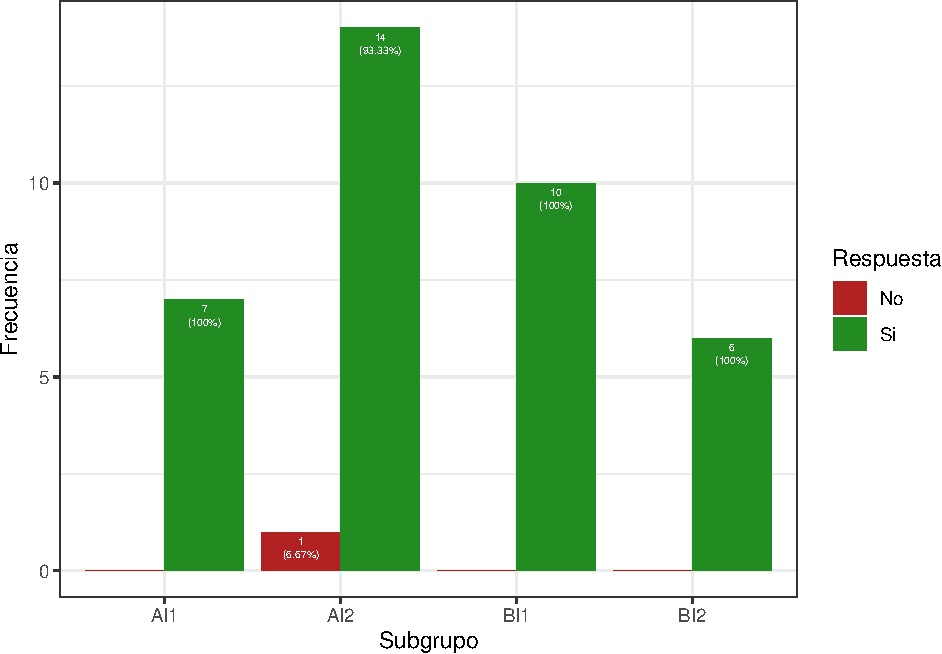
\includegraphics{informe_files/figure-latex/unnamed-chunk-11-1.pdf}

\hypertarget{uxedtem-11-en-el-futuro-recurriruxedas-a-o}{%
\section{\texorpdfstring{Ítem 11: En el futuro, ¿recurrirías a
\texttt{Word} o
\texttt{R Markdown}?}{Ítem 11: En el futuro, ¿recurrirías a  o ?}}\label{uxedtem-11-en-el-futuro-recurriruxedas-a-o}}

\begin{Shaded}
\begin{Highlighting}[]
\FunctionTok{levels}\NormalTok{(encuesta}\SpecialCharTok{$}\NormalTok{P11) }\OtherTok{\textless{}{-}} \FunctionTok{c}\NormalTok{(}\StringTok{"Word"}\NormalTok{, }\StringTok{"R Markdown"}\NormalTok{)}
\NormalTok{df11 }\OtherTok{\textless{}{-}} \FunctionTok{data.frame}\NormalTok{(}\AttributeTok{subgrupo =} \FunctionTok{rep}\NormalTok{(}\FunctionTok{levels}\NormalTok{(encuesta}\SpecialCharTok{$}\NormalTok{P1), }\AttributeTok{each =} \FunctionTok{length}\NormalTok{(}\FunctionTok{levels}\NormalTok{(encuesta}\SpecialCharTok{$}\NormalTok{P11))),}
                   \AttributeTok{respuesta =} \FunctionTok{rep}\NormalTok{(}\FunctionTok{levels}\NormalTok{(encuesta}\SpecialCharTok{$}\NormalTok{P11), }\AttributeTok{times =} \FunctionTok{length}\NormalTok{(}\FunctionTok{levels}\NormalTok{(encuesta}\SpecialCharTok{$}\NormalTok{P1))),}
                   \AttributeTok{frecuencia =} \FunctionTok{as.numeric}\NormalTok{(}\FunctionTok{unlist}\NormalTok{(}\FunctionTok{by}\NormalTok{(encuesta}\SpecialCharTok{$}\NormalTok{P11, encuesta}\SpecialCharTok{$}\NormalTok{P1, table))))}
\NormalTok{df11}\SpecialCharTok{$}\NormalTok{porcentaje }\OtherTok{\textless{}{-}} \FunctionTok{paste0}\NormalTok{(}\StringTok{"("}\NormalTok{, }\FunctionTok{round}\NormalTok{(}\FunctionTok{as.numeric}\NormalTok{(}\FunctionTok{unlist}\NormalTok{(}\FunctionTok{by}\NormalTok{(encuesta}\SpecialCharTok{$}\NormalTok{P11, encuesta}\SpecialCharTok{$}\NormalTok{P1, }\ControlFlowTok{function}\NormalTok{(x) \{}\FunctionTok{table}\NormalTok{(x)}\SpecialCharTok{/}\FunctionTok{sum}\NormalTok{(}\FunctionTok{table}\NormalTok{(x))\}))) }\SpecialCharTok{*} \DecValTok{100}\NormalTok{, }\DecValTok{2}\NormalTok{), }\StringTok{"\%"}\NormalTok{, }\StringTok{")"}\NormalTok{)}
\NormalTok{df11}
\end{Highlighting}
\end{Shaded}

\begin{verbatim}
##   subgrupo  respuesta frecuencia porcentaje
## 1      BI1       Word          2   (16.67%)
## 2      BI1 R Markdown         10   (83.33%)
## 3      BI2       Word          2      (25%)
## 4      BI2 R Markdown          6      (75%)
## 5      AI1       Word          0       (0%)
## 6      AI1 R Markdown          7     (100%)
## 7      AI2       Word         10   (55.56%)
## 8      AI2 R Markdown          8   (44.44%)
\end{verbatim}

\begin{Shaded}
\begin{Highlighting}[]
\NormalTok{p }\OtherTok{\textless{}{-}} \FunctionTok{ggplot}\NormalTok{(}\AttributeTok{data =}\NormalTok{ df11, }\FunctionTok{aes}\NormalTok{(}\AttributeTok{x =}\NormalTok{ subgrupo, }\AttributeTok{y =}\NormalTok{ frecuencia, }\AttributeTok{fill =}\NormalTok{ respuesta)) }\SpecialCharTok{+} 
  \FunctionTok{geom\_bar}\NormalTok{(}\AttributeTok{stat =} \StringTok{"identity"}\NormalTok{, }\AttributeTok{position=}\FunctionTok{position\_dodge}\NormalTok{()) }\SpecialCharTok{+}
  \FunctionTok{theme\_bw}\NormalTok{() }\SpecialCharTok{+} \FunctionTok{labs}\NormalTok{(}\AttributeTok{x =} \StringTok{"Subgrupo"}\NormalTok{, }\AttributeTok{y =} \StringTok{"Frecuencia"}\NormalTok{, }\AttributeTok{fill =} \StringTok{"Respuesta"}\NormalTok{) }\SpecialCharTok{+}
  \FunctionTok{geom\_text}\NormalTok{(}\FunctionTok{aes}\NormalTok{(}\AttributeTok{label =}\NormalTok{ frecuencia), }\AttributeTok{vjust =} \FloatTok{1.75}\NormalTok{, }\AttributeTok{position =} \FunctionTok{position\_dodge}\NormalTok{(}\FloatTok{0.9}\NormalTok{), }
            \AttributeTok{color =} \StringTok{"white"}\NormalTok{, }\AttributeTok{size =} \FloatTok{2.75}\NormalTok{) }\SpecialCharTok{+}
  \FunctionTok{geom\_text}\NormalTok{(}\FunctionTok{aes}\NormalTok{(}\AttributeTok{label =}\NormalTok{ porcentaje), }\AttributeTok{vjust =} \FloatTok{3.5}\NormalTok{, }\AttributeTok{position =} \FunctionTok{position\_dodge}\NormalTok{(}\FloatTok{0.9}\NormalTok{), }
            \AttributeTok{color =} \StringTok{"white"}\NormalTok{, }\AttributeTok{size =} \FloatTok{2.75}\NormalTok{) }\SpecialCharTok{+}
  \FunctionTok{scale\_fill\_manual}\NormalTok{(}\AttributeTok{values =} \FunctionTok{c}\NormalTok{(}\StringTok{"Word"} \OtherTok{=} \StringTok{"steelblue"}\NormalTok{, }\StringTok{"R Markdown"} \OtherTok{=} \StringTok{"forestgreen"}\NormalTok{)) }\SpecialCharTok{+}
  \FunctionTok{scale\_y\_continuous}\NormalTok{(}\AttributeTok{breaks =} \FunctionTok{seq}\NormalTok{(}\DecValTok{0}\NormalTok{, }\DecValTok{10}\NormalTok{, }\AttributeTok{by =} \DecValTok{2}\NormalTok{))}
\NormalTok{p}
\end{Highlighting}
\end{Shaded}

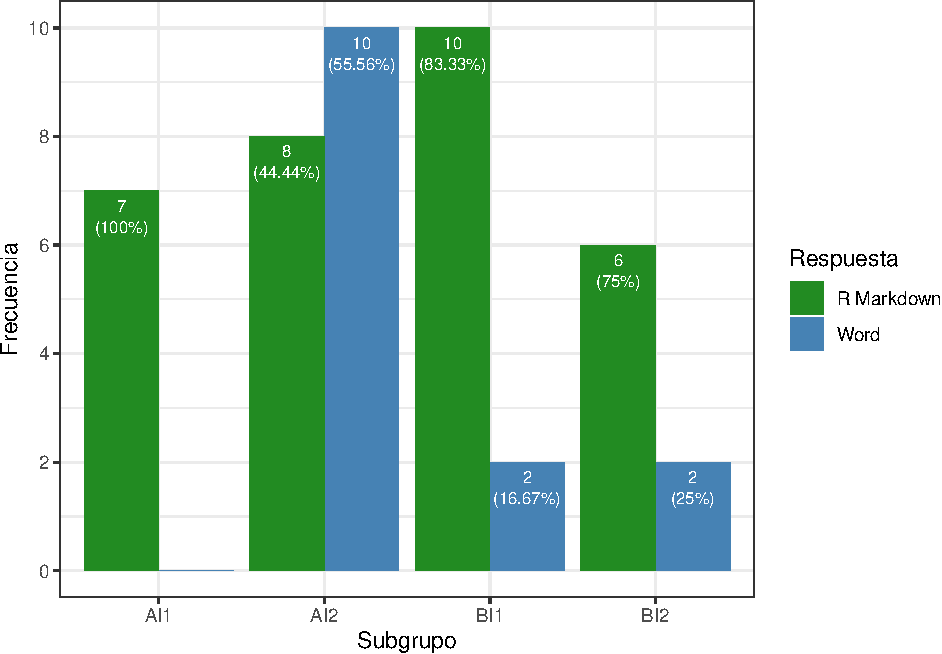
\includegraphics{informe_files/figure-latex/unnamed-chunk-12-1.pdf}

\hypertarget{uxedtem-12-recomendaruxedas-el-aprendizaje-de}{%
\section{\texorpdfstring{Ítem 12: ¿Recomendarías el aprendizaje de
\texttt{R Markdown}?}{Ítem 12: ¿Recomendarías el aprendizaje de ?}}\label{uxedtem-12-recomendaruxedas-el-aprendizaje-de}}

\begin{Shaded}
\begin{Highlighting}[]
\NormalTok{df12 }\OtherTok{\textless{}{-}} \FunctionTok{data.frame}\NormalTok{(}\AttributeTok{subgrupo =} \FunctionTok{rep}\NormalTok{(}\FunctionTok{levels}\NormalTok{(encuesta}\SpecialCharTok{$}\NormalTok{P1), }\AttributeTok{each =} \FunctionTok{length}\NormalTok{(}\FunctionTok{levels}\NormalTok{(encuesta}\SpecialCharTok{$}\NormalTok{P12))),}
                   \AttributeTok{respuesta =} \FunctionTok{rep}\NormalTok{(}\FunctionTok{levels}\NormalTok{(encuesta}\SpecialCharTok{$}\NormalTok{P12), }\AttributeTok{times =} \FunctionTok{length}\NormalTok{(}\FunctionTok{levels}\NormalTok{(encuesta}\SpecialCharTok{$}\NormalTok{P1))),}
                   \AttributeTok{frecuencia =} \FunctionTok{as.numeric}\NormalTok{(}\FunctionTok{unlist}\NormalTok{(}\FunctionTok{by}\NormalTok{(encuesta}\SpecialCharTok{$}\NormalTok{P12, encuesta}\SpecialCharTok{$}\NormalTok{P1, table))))}
\NormalTok{df12}\SpecialCharTok{$}\NormalTok{porcentaje }\OtherTok{\textless{}{-}} \FunctionTok{paste0}\NormalTok{(}\StringTok{"("}\NormalTok{, }\FunctionTok{round}\NormalTok{(}\FunctionTok{as.numeric}\NormalTok{(}\FunctionTok{unlist}\NormalTok{(}\FunctionTok{by}\NormalTok{(encuesta}\SpecialCharTok{$}\NormalTok{P12, encuesta}\SpecialCharTok{$}\NormalTok{P1, }\ControlFlowTok{function}\NormalTok{(x) \{}\FunctionTok{table}\NormalTok{(x)}\SpecialCharTok{/}\FunctionTok{sum}\NormalTok{(}\FunctionTok{table}\NormalTok{(x))\}))) }\SpecialCharTok{*} \DecValTok{100}\NormalTok{, }\DecValTok{2}\NormalTok{), }\StringTok{"\%"}\NormalTok{, }\StringTok{")"}\NormalTok{)}
\NormalTok{df12}
\end{Highlighting}
\end{Shaded}

\begin{verbatim}
##   subgrupo respuesta frecuencia porcentaje
## 1      BI1        No          0       (0%)
## 2      BI1        Si         12     (100%)
## 3      BI2        No          0       (0%)
## 4      BI2        Si          7     (100%)
## 5      AI1        No          0       (0%)
## 6      AI1        Si          6     (100%)
## 7      AI2        No          1    (7.69%)
## 8      AI2        Si         12   (92.31%)
\end{verbatim}

\begin{Shaded}
\begin{Highlighting}[]
\NormalTok{p }\OtherTok{\textless{}{-}} \FunctionTok{ggplot}\NormalTok{(}\AttributeTok{data =}\NormalTok{ df12, }\FunctionTok{aes}\NormalTok{(}\AttributeTok{x =}\NormalTok{ subgrupo, }\AttributeTok{y =}\NormalTok{ frecuencia, }\AttributeTok{fill =}\NormalTok{ respuesta)) }\SpecialCharTok{+} 
  \FunctionTok{geom\_bar}\NormalTok{(}\AttributeTok{stat =} \StringTok{"identity"}\NormalTok{, }\AttributeTok{position=}\FunctionTok{position\_dodge}\NormalTok{()) }\SpecialCharTok{+}
  \FunctionTok{theme\_bw}\NormalTok{() }\SpecialCharTok{+} \FunctionTok{labs}\NormalTok{(}\AttributeTok{x =} \StringTok{"Subgrupo"}\NormalTok{, }\AttributeTok{y =} \StringTok{"Frecuencia"}\NormalTok{, }\AttributeTok{fill =} \StringTok{"Respuesta"}\NormalTok{) }\SpecialCharTok{+}
  \FunctionTok{geom\_text}\NormalTok{(}\FunctionTok{aes}\NormalTok{(}\AttributeTok{label =}\NormalTok{ frecuencia), }\AttributeTok{vjust =} \FloatTok{1.75}\NormalTok{, }\AttributeTok{position =} \FunctionTok{position\_dodge}\NormalTok{(}\FloatTok{0.9}\NormalTok{), }
            \AttributeTok{color =} \StringTok{"white"}\NormalTok{, }\AttributeTok{size =} \FloatTok{1.75}\NormalTok{) }\SpecialCharTok{+}
  \FunctionTok{geom\_text}\NormalTok{(}\FunctionTok{aes}\NormalTok{(}\AttributeTok{label =}\NormalTok{ porcentaje), }\AttributeTok{vjust =} \FloatTok{3.5}\NormalTok{, }\AttributeTok{position =} \FunctionTok{position\_dodge}\NormalTok{(}\FloatTok{0.9}\NormalTok{), }
            \AttributeTok{color =} \StringTok{"white"}\NormalTok{, }\AttributeTok{size =} \FloatTok{1.75}\NormalTok{) }\SpecialCharTok{+}
  \FunctionTok{scale\_fill\_manual}\NormalTok{(}\AttributeTok{values =} \FunctionTok{c}\NormalTok{(}\StringTok{"No"} \OtherTok{=} \StringTok{"firebrick"}\NormalTok{, }\StringTok{"Si"} \OtherTok{=} \StringTok{"forestgreen"}\NormalTok{)) }\SpecialCharTok{+}
  \FunctionTok{scale\_y\_continuous}\NormalTok{(}\AttributeTok{breaks =} \FunctionTok{seq}\NormalTok{(}\DecValTok{0}\NormalTok{, }\DecValTok{12}\NormalTok{, }\AttributeTok{by =} \DecValTok{3}\NormalTok{))}
\NormalTok{p}
\end{Highlighting}
\end{Shaded}

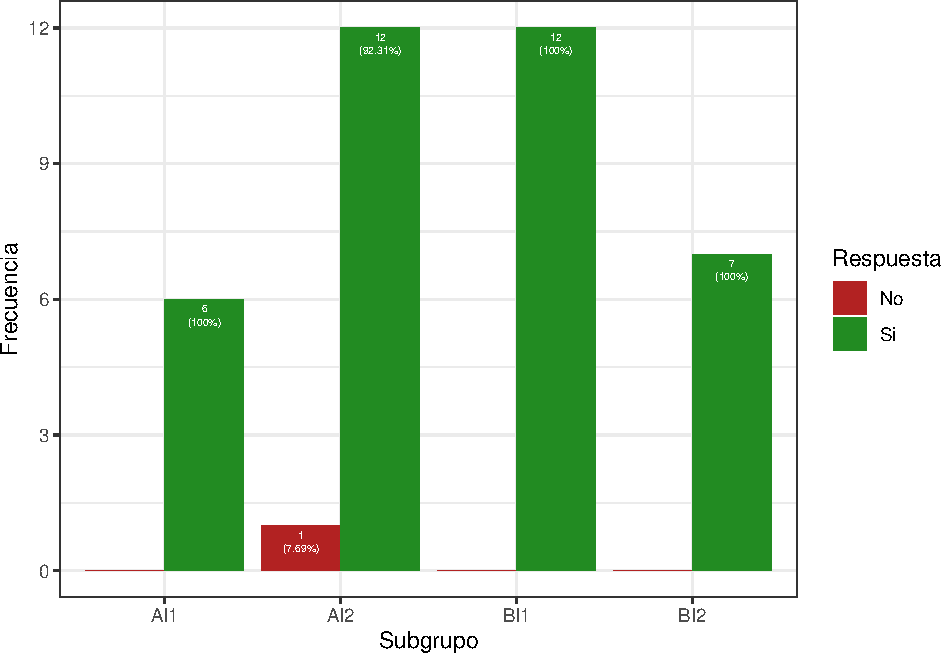
\includegraphics{informe_files/figure-latex/unnamed-chunk-13-1.pdf}

\hypertarget{uxedtem-13-lo-que-muxe1s-me-ha-gustado-de-es}{%
\section{\texorpdfstring{Ítem 13: Lo que más me ha gustado de
\texttt{R Markdown}
es\ldots{}}{Ítem 13: Lo que más me ha gustado de  es\ldots{}}}\label{uxedtem-13-lo-que-muxe1s-me-ha-gustado-de-es}}

\begin{Shaded}
\begin{Highlighting}[]
\CommentTok{\# Vector de texto}
\NormalTok{encuesta}\SpecialCharTok{$}\NormalTok{P13}
\end{Highlighting}
\end{Shaded}

\begin{verbatim}
##  [1] "Las salidas que daba eran bastante intuitivas y fáciles de comprender"                                                                                                                                                                                                      
##  [2] "Me gustan los colorines de las gráficas"                                                                                                                                                                                                                                    
##  [3] "Simplifica mucho hacer los cálculos y los test."                                                                                                                                                                                                                            
##  [4] "La facilidad de realizar los tests"                                                                                                                                                                                                                                         
##  [5] "Que tanto la instrucción  como el resultado se copia al instante, es mucho más rápido que si hubiera que copiarlo en otro documento. "                                                                                                                                      
##  [6] "Poder generar informes de manera más rápida y sencilla"                                                                                                                                                                                                                     
##  [7] NA                                                                                                                                                                                                                                                                           
##  [8] "Creo que si sabes usarlo bien puede ser muy útil."                                                                                                                                                                                                                          
##  [9] NA                                                                                                                                                                                                                                                                           
## [10] "sobre todo molan los gráficos que son muy utiles"                                                                                                                                                                                                                           
## [11] "Que puedas tanto escribir en el texto como mantener el formato de programación., a diferencia de copiar y pegar/ agregar imágenes en Word."                                                                                                                                 
## [12] "Me parece un programa muy intuitivo"                                                                                                                                                                                                                                        
## [13] "La versatilidad del programa a la hora de realizar análisis y rellenar informes"                                                                                                                                                                                            
## [14] "Me ha ayudado bastante a la hora de entender la teoría y los problemas de la asignatura."                                                                                                                                                                                   
## [15] "Al principio al ser nuevo costo un poco adaptarse al lenguaje del programa y todas las opciones. Pero al final logré controlarlo relativamente bien y fue bastante interesante."                                                                                            
## [16] "Facilidad para obtener análisis."                                                                                                                                                                                                                                           
## [17] "La forma en la que los profesores la habéis impartido ( ya que he asistido a clases de ambos grupos), la forma en que la teoría se aplica a la práctica , la utilidad de esto en el examen."                                                                                
## [18] "Lo que más me ha gustado es su comodidad, ya que desde el programa R puedo ir haciendo el informe e ir poniendo las diferentes salidas, y al final me lo puedo descargar para ver todos los pasos que he seguido durante la práctica. Muy satisfecha."                      
## [19] "Solo necesitas escribir en R, no hay que escribir todo dos veces y las gráficas y el codigo sale automaticamente en el R markdown. N necesito copiar y pegar cosas. También se puede copiar y pegar el codigo dentro de R. Es muy bien organizado el fichero de R markdown."
## [20] "Me ha gustado todos "                                                                                                                                                                                                                                                       
## [21] "Queda guardat i pots veure la pràctica que has fet, i obrir-la al R per completar o canviar. Les gràfiques ixen directament al document, es fa tot més ràpid."                                                                                                              
## [22] "És molt útil per a cohesionar les explicacions (teòriques com els contrastos d'hipòtesis) amb les eixides del R (script), de forma que no has d'anar fent captura de pantalla i enganxar-ho al Word."                                                                       
## [23] NA                                                                                                                                                                                                                                                                           
## [24] NA                                                                                                                                                                                                                                                                           
## [25] NA                                                                                                                                                                                                                                                                           
## [26] NA                                                                                                                                                                                                                                                                           
## [27] NA                                                                                                                                                                                                                                                                           
## [28] "La facilitat per generar gràfiques de les dades."                                                                                                                                                                                                                           
## [29] NA                                                                                                                                                                                                                                                                           
## [30] NA                                                                                                                                                                                                                                                                           
## [31] "La facilitat de lectura"                                                                                                                                                                                                                                                    
## [32] NA                                                                                                                                                                                                                                                                           
## [33] NA                                                                                                                                                                                                                                                                           
## [34] "La facilitat que dona per a analitzar dades estadístiques."                                                                                                                                                                                                                 
## [35] NA                                                                                                                                                                                                                                                                           
## [36] NA                                                                                                                                                                                                                                                                           
## [37] "res"                                                                                                                                                                                                                                                                        
## [38] "Veure els diagrames, són molt explicatius i útils. També m'ha agradat vore com un problema de classe es pot resoldre amb un programa informàtic."                                                                                                                           
## [39] "els gràfics"                                                                                                                                                                                                                                                                
## [40] "Que pots veure els gràfics, i això es molt visual."                                                                                                                                                                                                                         
## [41] "La facilitat de compendre els conceptes i els resultats. "                                                                                                                                                                                                                  
## [42] "El fet de poder fer informes de manera tan senzilla i aportant dades estadístiques directament des del programa, a l'igual que les gràfiques, etc. "                                                                                                                        
## [43] "-"                                                                                                                                                                                                                                                                          
## [44] NA                                                                                                                                                                                                                                                                           
## [45] "Es intuitivo. "                                                                                                                                                                                                                                                             
## [46] NA                                                                                                                                                                                                                                                                           
## [47] NA
\end{verbatim}

\begin{Shaded}
\begin{Highlighting}[]
\NormalTok{text\_vector }\OtherTok{\textless{}{-}} \FunctionTok{c}\NormalTok{(}
  \StringTok{"Las salidas que daba eran bastante intuitivas y fáciles de comprender"}\NormalTok{,}
  \StringTok{"Me gustan los colores de las gráficas"}\NormalTok{,}
  \StringTok{"Simplifica mucho hacer los cálculos y los test"}\NormalTok{,}
  \StringTok{"La facilidad para realizar los test"}\NormalTok{,}
  \StringTok{"Que tanto la instrucción como el resultado se copian al instante; es mucho más rápido que si hubiera que hacerlo en otro documento"}\NormalTok{,}
  \StringTok{"Poder generar informes de manera más rápida y sencilla"}\NormalTok{,}
  \ConstantTok{NA}\NormalTok{,}
  \StringTok{"Creo que, si sabes usarlo bien, puede ser muy útil"}\NormalTok{,}
  \ConstantTok{NA}\NormalTok{,}
  \StringTok{"Sobre todo, me gustan los gráficos, que son muy útiles"}\NormalTok{,}
  \StringTok{"Que puedas escribir texto y mantener el formato de programación, a diferencia de copiar, pegar o añadir imágenes en Word"}\NormalTok{,}
  \StringTok{"Me parece un programa muy intuitivo"}\NormalTok{,}
  \StringTok{"La versatilidad del programa para realizar análisis y redactar informes"}\NormalTok{,}
  \StringTok{"Me ha ayudado bastante a entender la teoría y los problemas de la asignatura"}\NormalTok{,}
  \StringTok{"Al principio, al ser nuevo, costó un poco adaptarse al lenguaje del programa y a todas sus opciones. Pero al final logré controlarlo relativamente bien y fue bastante interesante"}\NormalTok{,}
  \StringTok{"Facilidad para obtener análisis"}\NormalTok{,}
  \StringTok{"La forma en que los profesores lo habéis impartido (he asistido a clases de ambos grupos), cómo la teoría se aplica a la práctica y su utilidad para el examen"}\NormalTok{,}
  \StringTok{"Lo que más me ha gustado es su comodidad: desde R puedo ir haciendo el informe, añadiendo las salidas, y al final descargarlo para ver todos los pasos seguidos durante la práctica. Muy satisfecha"}\NormalTok{,}
  \StringTok{"Solo necesitas escribir en R; no hay que repetir todo, y las gráficas y el código aparecen automáticamente en R Markdown. No necesito copiar y pegar nada. También se puede copiar y pegar el código dentro de R. El fichero de R Markdown está muy bien organizado"}\NormalTok{,}
  \StringTok{"Me ha gustado todo"}\NormalTok{,}
  \StringTok{"Queda guardado y puedes ver la práctica que has hecho y abrirla en R para completarla o modificarla. Las gráficas aparecen directamente en el documento, todo es más rápido"}\NormalTok{,}
  \StringTok{"Es muy útil para integrar las explicaciones (teóricas como los contrastes de hipótesis) con las salidas de R (script), de forma que no tienes que hacer capturas de pantalla ni pegarlas en Word"}\NormalTok{,}
  \ConstantTok{NA}\NormalTok{,}
  \ConstantTok{NA}\NormalTok{,}
  \ConstantTok{NA}\NormalTok{,}
  \ConstantTok{NA}\NormalTok{,}
  \ConstantTok{NA}\NormalTok{,}
  \StringTok{"La facilidad para generar gráficas a partir de los datos"}\NormalTok{,}
  \ConstantTok{NA}\NormalTok{,}
  \ConstantTok{NA}\NormalTok{,}
  \StringTok{"La facilidad de lectura"}\NormalTok{,}
  \ConstantTok{NA}\NormalTok{,}
  \ConstantTok{NA}\NormalTok{,}
  \StringTok{"La facilidad que ofrece para analizar datos estadísticos"}\NormalTok{,}
  \ConstantTok{NA}\NormalTok{,}
  \ConstantTok{NA}\NormalTok{,}
  \StringTok{"Nada"}\NormalTok{,}
  \StringTok{"Ver los diagramas, que son muy explicativos y útiles. También me ha gustado ver cómo un problema de clase se puede resolver con un programa informático"}\NormalTok{,}
  \StringTok{"Los gráficos"}\NormalTok{,}
  \StringTok{"Que puedes ver los gráficos, y eso es muy visual"}\NormalTok{,}
  \StringTok{"La facilidad para comprender los conceptos y los resultados"}\NormalTok{,}
  \StringTok{"El hecho de poder hacer informes de forma tan sencilla, incluyendo datos estadísticos y gráficas directamente desde el programa"}\NormalTok{,}
  \ConstantTok{NA}\NormalTok{,}
  \ConstantTok{NA}\NormalTok{,}
  \StringTok{"Es intuitivo"}\NormalTok{,}
  \ConstantTok{NA}\NormalTok{,}
  \ConstantTok{NA}
\NormalTok{)}

\CommentTok{\# Convierte a un corpus}
\NormalTok{corpus }\OtherTok{\textless{}{-}} \FunctionTok{Corpus}\NormalTok{(}\FunctionTok{VectorSource}\NormalTok{(text\_vector))}

\CommentTok{\# Limpieza básica del texto}
\NormalTok{corpus }\OtherTok{\textless{}{-}} \FunctionTok{tm\_map}\NormalTok{(corpus, removePunctuation)                    }\CommentTok{\# elimina puntuación}
\end{Highlighting}
\end{Shaded}

\begin{verbatim}
## Warning in tm_map.SimpleCorpus(corpus, removePunctuation): transformation drops
## documents
\end{verbatim}

\begin{Shaded}
\begin{Highlighting}[]
\NormalTok{corpus }\OtherTok{\textless{}{-}} \FunctionTok{tm\_map}\NormalTok{(corpus, }\FunctionTok{content\_transformer}\NormalTok{(tolower))         }\CommentTok{\# a minúsculas}
\end{Highlighting}
\end{Shaded}

\begin{verbatim}
## Warning in tm_map.SimpleCorpus(corpus, content_transformer(tolower)):
## transformation drops documents
\end{verbatim}

\begin{Shaded}
\begin{Highlighting}[]
\NormalTok{corpus }\OtherTok{\textless{}{-}} \FunctionTok{tm\_map}\NormalTok{(corpus, removeNumbers)                        }\CommentTok{\# elimina números}
\end{Highlighting}
\end{Shaded}

\begin{verbatim}
## Warning in tm_map.SimpleCorpus(corpus, removeNumbers): transformation drops
## documents
\end{verbatim}

\begin{Shaded}
\begin{Highlighting}[]
\NormalTok{corpus }\OtherTok{\textless{}{-}} \FunctionTok{tm\_map}\NormalTok{(corpus, stripWhitespace)                      }\CommentTok{\# elimina muchos espacios}
\end{Highlighting}
\end{Shaded}

\begin{verbatim}
## Warning in tm_map.SimpleCorpus(corpus, stripWhitespace): transformation drops
## documents
\end{verbatim}

\begin{Shaded}
\begin{Highlighting}[]
\NormalTok{corpus }\OtherTok{\textless{}{-}} \FunctionTok{tm\_map}\NormalTok{(corpus, removeWords, }\FunctionTok{stopwords}\NormalTok{(}\StringTok{"spanish"}\NormalTok{))    }\CommentTok{\# elimina stopwords en español}
\end{Highlighting}
\end{Shaded}

\begin{verbatim}
## Warning in tm_map.SimpleCorpus(corpus, removeWords, stopwords("spanish")):
## transformation drops documents
\end{verbatim}

\begin{Shaded}
\begin{Highlighting}[]
\CommentTok{\# wordcloud(corpus, scale = c(2, 1), min.freq = 3, colors = rainbow(30))}

\CommentTok{\# Crear matriz de términos}
\NormalTok{tdm }\OtherTok{\textless{}{-}} \FunctionTok{TermDocumentMatrix}\NormalTok{(corpus)}
\NormalTok{m }\OtherTok{\textless{}{-}} \FunctionTok{as.matrix}\NormalTok{(tdm)}
\NormalTok{word\_freqs }\OtherTok{\textless{}{-}} \FunctionTok{sort}\NormalTok{(}\FunctionTok{rowSums}\NormalTok{(m), }\AttributeTok{decreasing =} \ConstantTok{TRUE}\NormalTok{)}

\CommentTok{\# Dibujar la nube}
\FunctionTok{par}\NormalTok{(}\AttributeTok{mar =} \FunctionTok{c}\NormalTok{(}\DecValTok{1}\NormalTok{, }\DecValTok{1}\NormalTok{, }\DecValTok{1}\NormalTok{, }\DecValTok{1}\NormalTok{))}
\FunctionTok{wordcloud}\NormalTok{(}\FunctionTok{names}\NormalTok{(word\_freqs), }\AttributeTok{scale =} \FunctionTok{c}\NormalTok{(}\DecValTok{2}\NormalTok{, }\FloatTok{0.75}\NormalTok{), word\_freqs, }\AttributeTok{min.freq =} \DecValTok{2}\NormalTok{, }
          \AttributeTok{colors =} \FunctionTok{rainbow}\NormalTok{(}\DecValTok{30}\NormalTok{))}
\end{Highlighting}
\end{Shaded}

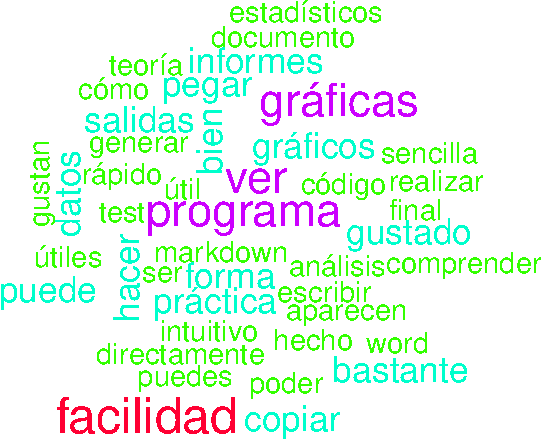
\includegraphics{informe_files/figure-latex/unnamed-chunk-14-1.pdf}

\hypertarget{uxedtem-14-lo-que-menos-me-ha-gustado-de-es}{%
\section{\texorpdfstring{Ítem 14: Lo que menos me ha gustado de
\texttt{R Markdown}
es\ldots{}}{Ítem 14: Lo que menos me ha gustado de  es\ldots{}}}\label{uxedtem-14-lo-que-menos-me-ha-gustado-de-es}}

\begin{Shaded}
\begin{Highlighting}[]
\CommentTok{\# Vector de texto}
\NormalTok{encuesta}\SpecialCharTok{$}\NormalTok{P14}
\end{Highlighting}
\end{Shaded}

\begin{verbatim}
##  [1] "Algunos comandos eran complejos"                                                                                                                                                                                                                                                                                                                                                                        
##  [2] "no me gustan las gráficas sin colores"                                                                                                                                                                                                                                                                                                                                                                  
##  [3] "que a veces no sabíamos generar informes o daba problemas o se quedaba pillado."                                                                                                                                                                                                                                                                                                                        
##  [4] "La dificultad para organizar el informe ya que copiar pegar y los tests que se ponen al final"                                                                                                                                                                                                                                                                                                          
##  [5] "Puede ser un poco lioso a la hora de ordenar el documento."                                                                                                                                                                                                                                                                                                                                             
##  [6] "Que al realizar informes al realizar pruebas y tests estadísticos quedaban en la parte más inferior, pero me parece mejor que Word."                                                                                                                                                                                                                                                                    
##  [7] NA                                                                                                                                                                                                                                                                                                                                                                                                       
##  [8] "No siempre tener claros los pasos y atascarme en la tarea."                                                                                                                                                                                                                                                                                                                                             
##  [9] NA                                                                                                                                                                                                                                                                                                                                                                                                       
## [10] "Si no sabes qué tests hacer es un poco dificil"                                                                                                                                                                                                                                                                                                                                                         
## [11] "tener que revisar constantemente si lo que escribí se había generado o no, debería haber una opción que permita realizar esto mas fácilmente."                                                                                                                                                                                                                                                          
## [12] "A veces  las opciones eran un poco confusas"                                                                                                                                                                                                                                                                                                                                                            
## [13] "Al principio es frustrante entenderlo y los comandos no son intuitivos"                                                                                                                                                                                                                                                                                                                                 
## [14] "Es un poco frustrante que haya \"atajos\" para ciertas funciones pero no para todas, porque a la hora de escribir comandos por mucho que estén en la presentación al no habernos explicado como escribirlos y como funciona el lenguaje de R (si admite ciertos signos, tildes, etc.) se hace complicado y casi siempre requiere la ayuda del profesor lo cual rompe un poco la dinámica del ejercicio."
## [15] NA                                                                                                                                                                                                                                                                                                                                                                                                       
## [16] NA                                                                                                                                                                                                                                                                                                                                                                                                       
## [17] "No encuentro nada negativo"                                                                                                                                                                                                                                                                                                                                                                             
## [18] NA                                                                                                                                                                                                                                                                                                                                                                                                       
## [19] "En R es facil perderse dentro del codigo y hace que a veces es un poco complicado cambiar lo que quieres que salga en el R markdown."                                                                                                                                                                                                                                                                   
## [20] "No me ha gustado es cuando tuve que usarlo en mi computadora porque era diferente al que tenía en la práctica."                                                                                                                                                                                                                                                                                         
## [21] "Quan escriues en una sola línia continua, a partir de certa longitud del text no pots veure el final de la frase, pel que dificulta poder vore els excercisis al programa sense generar un informe."                                                                                                                                                                                                    
## [22] "A nivell d'estil, que no se veu tot el text a la mateixa pantalla, has de desplaçar-te horitzontalment. I de voltes mareja ja que no saps si estàs escrivint o no i què. I tampoc pots veure les dades a les que t'has referit de forma simultània."                                                                                                                                                    
## [23] NA                                                                                                                                                                                                                                                                                                                                                                                                       
## [24] NA                                                                                                                                                                                                                                                                                                                                                                                                       
## [25] NA                                                                                                                                                                                                                                                                                                                                                                                                       
## [26] NA                                                                                                                                                                                                                                                                                                                                                                                                       
## [27] NA                                                                                                                                                                                                                                                                                                                                                                                                       
## [28] "La interfaç poc intuitiva."                                                                                                                                                                                                                                                                                                                                                                             
## [29] NA                                                                                                                                                                                                                                                                                                                                                                                                       
## [30] NA                                                                                                                                                                                                                                                                                                                                                                                                       
## [31] "Els gràfics de l'examen"                                                                                                                                                                                                                                                                                                                                                                                
## [32] NA                                                                                                                                                                                                                                                                                                                                                                                                       
## [33] NA                                                                                                                                                                                                                                                                                                                                                                                                       
## [34] "A vegades costa relacionar el que demana en l'exercici amb lo que he d'emprar en R."                                                                                                                                                                                                                                                                                                                    
## [35] NA                                                                                                                                                                                                                                                                                                                                                                                                       
## [36] NA                                                                                                                                                                                                                                                                                                                                                                                                       
## [37] "no s'enten"                                                                                                                                                                                                                                                                                                                                                                                             
## [38] "Hi ha vegades que no funciona bé i que o no genera l'informe o no es transcriuen les dades del fitxer."                                                                                                                                                                                                                                                                                                 
## [39] NA                                                                                                                                                                                                                                                                                                                                                                                                       
## [40] "La dificultat per aprender-ho, ja que hi havia vegades que no era molt intuitiu."                                                                                                                                                                                                                                                                                                                       
## [41] "La dificultat que hi havia a voltes de poder arribar a trobar el mètode a executar en el programa. "                                                                                                                                                                                                                                                                                                    
## [42] NA                                                                                                                                                                                                                                                                                                                                                                                                       
## [43] "-"                                                                                                                                                                                                                                                                                                                                                                                                      
## [44] NA                                                                                                                                                                                                                                                                                                                                                                                                       
## [45] "Creo que es más útil Excel, tanto para análisis estadísticos como para otras opciones. "                                                                                                                                                                                                                                                                                                                
## [46] NA                                                                                                                                                                                                                                                                                                                                                                                                       
## [47] NA
\end{verbatim}

\begin{Shaded}
\begin{Highlighting}[]
\NormalTok{text\_vector }\OtherTok{\textless{}{-}} \FunctionTok{c}\NormalTok{(}
  \StringTok{"Algunos comandos eran complejos"}\NormalTok{,}
  \StringTok{"No me gustan las gráficas sin colores"}\NormalTok{,}
  \StringTok{"Que a veces no sabíamos generar informes o daba problemas o se quedaba pillado"}\NormalTok{,}
  \StringTok{"La dificultad para organizar el informe, ya que copiar y pegar y los tests se ponen al final"}\NormalTok{,}
  \StringTok{"Puede ser un poco lioso a la hora de ordenar el documento"}\NormalTok{,}
  \StringTok{"Que al realizar informes y pruebas estadísticas, los resultados quedaban en la parte inferior, aunque me parece mejor que Word"}\NormalTok{,}
  \ConstantTok{NA}\NormalTok{,}
  \StringTok{"No siempre tenía claros los pasos y me atascaba en la tarea"}\NormalTok{,}
  \ConstantTok{NA}\NormalTok{,}
  \StringTok{"Si no sabes qué test hacer, es un poco difícil"}\NormalTok{,}
  \StringTok{"Tener que revisar constantemente si lo que escribí se había generado o no; debería haber una opción que permitiera hacer esto más fácilmente"}\NormalTok{,}
  \StringTok{"A veces las opciones eran un poco confusas"}\NormalTok{,}
  \StringTok{"Al principio es frustrante entenderlo y los comandos no son intuitivos"}\NormalTok{,}
  \StringTok{"Es frustrante que haya atajos para ciertas funciones pero no para todas, porque aunque estén en la presentación, al no explicarnos cómo escribirlos ni cómo funciona el lenguaje de R (si admite ciertos signos, tildes, etc.), se hace complicado y casi siempre se requiere la ayuda del profesor, lo cual rompe la dinámica del ejercicio"}\NormalTok{,}
  \ConstantTok{NA}\NormalTok{,}
  \ConstantTok{NA}\NormalTok{,}
  \StringTok{"No encuentro nada negativo"}\NormalTok{,}
  \ConstantTok{NA}\NormalTok{,}
  \StringTok{"En R es fácil perderse en el código y a veces es complicado cambiar lo que quieres que aparezca en el R Markdown"}\NormalTok{,}
  \StringTok{"No me gustó cuando tuve que usarlo en mi ordenador porque era diferente al de las prácticas"}\NormalTok{,}
  \StringTok{"Cuando escribes en una sola línea continua, a partir de cierta longitud no puedes ver el final de la frase, lo que dificulta ver los ejercicios sin generar el informe"}\NormalTok{,}
  \StringTok{"A nivel de estilo, no se ve todo el texto en la misma pantalla, tienes que desplazarte horizontalmente, y a veces marea porque no sabes si estás escribiendo o no ni qué. Tampoco puedes ver simultáneamente los datos a los que te refieres"}\NormalTok{,}
  \ConstantTok{NA}\NormalTok{,}
  \ConstantTok{NA}\NormalTok{,}
  \ConstantTok{NA}\NormalTok{,}
  \ConstantTok{NA}\NormalTok{,}
  \ConstantTok{NA}\NormalTok{,}
  \StringTok{"La interfaz es poco intuitiva"}\NormalTok{,}
  \ConstantTok{NA}\NormalTok{,}
  \ConstantTok{NA}\NormalTok{,}
  \StringTok{"Los gráficos del examen"}\NormalTok{,}
  \ConstantTok{NA}\NormalTok{,}
  \ConstantTok{NA}\NormalTok{,}
  \StringTok{"A veces cuesta relacionar lo que pide el ejercicio con lo que hay que usar en R"}\NormalTok{,}
  \ConstantTok{NA}\NormalTok{,}
  \ConstantTok{NA}\NormalTok{,}
  \StringTok{"No se entiende"}\NormalTok{,}
  \StringTok{"A veces no funciona bien: no genera el informe o no se transcriben los datos del fichero"}\NormalTok{,}
  \ConstantTok{NA}\NormalTok{,}
  \StringTok{"La dificultad para aprenderlo, ya que a veces no era muy intuitivo"}\NormalTok{,}
  \StringTok{"La dificultad que había a veces para encontrar el método a ejecutar en el programa"}\NormalTok{,}
  \ConstantTok{NA}\NormalTok{,}
  \ConstantTok{NA}\NormalTok{,}
  \ConstantTok{NA}\NormalTok{,}
  \StringTok{"Creo que Excel es más útil, tanto para análisis estadísticos como para otras funciones"}\NormalTok{,}
  \ConstantTok{NA}\NormalTok{,}
  \ConstantTok{NA}
\NormalTok{)}

\CommentTok{\# Convierte a un corpus}
\NormalTok{corpus }\OtherTok{\textless{}{-}} \FunctionTok{Corpus}\NormalTok{(}\FunctionTok{VectorSource}\NormalTok{(text\_vector))}

\CommentTok{\# Limpieza básica del texto}
\NormalTok{corpus }\OtherTok{\textless{}{-}} \FunctionTok{tm\_map}\NormalTok{(corpus, removePunctuation)                    }\CommentTok{\# elimina puntuación}
\end{Highlighting}
\end{Shaded}

\begin{verbatim}
## Warning in tm_map.SimpleCorpus(corpus, removePunctuation): transformation drops
## documents
\end{verbatim}

\begin{Shaded}
\begin{Highlighting}[]
\NormalTok{corpus }\OtherTok{\textless{}{-}} \FunctionTok{tm\_map}\NormalTok{(corpus, }\FunctionTok{content\_transformer}\NormalTok{(tolower))         }\CommentTok{\# a minúsculas}
\end{Highlighting}
\end{Shaded}

\begin{verbatim}
## Warning in tm_map.SimpleCorpus(corpus, content_transformer(tolower)):
## transformation drops documents
\end{verbatim}

\begin{Shaded}
\begin{Highlighting}[]
\NormalTok{corpus }\OtherTok{\textless{}{-}} \FunctionTok{tm\_map}\NormalTok{(corpus, removeNumbers)                        }\CommentTok{\# elimina números}
\end{Highlighting}
\end{Shaded}

\begin{verbatim}
## Warning in tm_map.SimpleCorpus(corpus, removeNumbers): transformation drops
## documents
\end{verbatim}

\begin{Shaded}
\begin{Highlighting}[]
\NormalTok{corpus }\OtherTok{\textless{}{-}} \FunctionTok{tm\_map}\NormalTok{(corpus, stripWhitespace)                      }\CommentTok{\# elimina muchos espacios}
\end{Highlighting}
\end{Shaded}

\begin{verbatim}
## Warning in tm_map.SimpleCorpus(corpus, stripWhitespace): transformation drops
## documents
\end{verbatim}

\begin{Shaded}
\begin{Highlighting}[]
\NormalTok{corpus }\OtherTok{\textless{}{-}} \FunctionTok{tm\_map}\NormalTok{(corpus, removeWords, }\FunctionTok{stopwords}\NormalTok{(}\StringTok{"spanish"}\NormalTok{))    }\CommentTok{\# elimina stopwords en español}
\end{Highlighting}
\end{Shaded}

\begin{verbatim}
## Warning in tm_map.SimpleCorpus(corpus, removeWords, stopwords("spanish")):
## transformation drops documents
\end{verbatim}

\begin{Shaded}
\begin{Highlighting}[]
\NormalTok{corpus }\OtherTok{\textless{}{-}} \FunctionTok{tm\_map}\NormalTok{(corpus, removeWords, }\FunctionTok{c}\NormalTok{(}\StringTok{"veces"}\NormalTok{))}
\end{Highlighting}
\end{Shaded}

\begin{verbatim}
## Warning in tm_map.SimpleCorpus(corpus, removeWords, c("veces")): transformation
## drops documents
\end{verbatim}

\begin{Shaded}
\begin{Highlighting}[]
\CommentTok{\# Crear matriz de términos}
\NormalTok{tdm }\OtherTok{\textless{}{-}} \FunctionTok{TermDocumentMatrix}\NormalTok{(corpus)}
\NormalTok{m }\OtherTok{\textless{}{-}} \FunctionTok{as.matrix}\NormalTok{(tdm)}
\NormalTok{word\_freqs }\OtherTok{\textless{}{-}} \FunctionTok{sort}\NormalTok{(}\FunctionTok{rowSums}\NormalTok{(m), }\AttributeTok{decreasing =} \ConstantTok{TRUE}\NormalTok{)}

\CommentTok{\# Dibujar la nube}
\FunctionTok{par}\NormalTok{(}\AttributeTok{mar =} \FunctionTok{c}\NormalTok{(}\DecValTok{1}\NormalTok{, }\DecValTok{1}\NormalTok{, }\DecValTok{1}\NormalTok{, }\DecValTok{1}\NormalTok{))}
\FunctionTok{wordcloud}\NormalTok{(}\FunctionTok{names}\NormalTok{(word\_freqs), }\AttributeTok{scale =} \FunctionTok{c}\NormalTok{(}\DecValTok{2}\NormalTok{, }\FloatTok{0.75}\NormalTok{), word\_freqs, }\AttributeTok{min.freq =} \DecValTok{2}\NormalTok{, }
          \AttributeTok{colors =} \FunctionTok{rainbow}\NormalTok{(}\DecValTok{30}\NormalTok{))}
\end{Highlighting}
\end{Shaded}

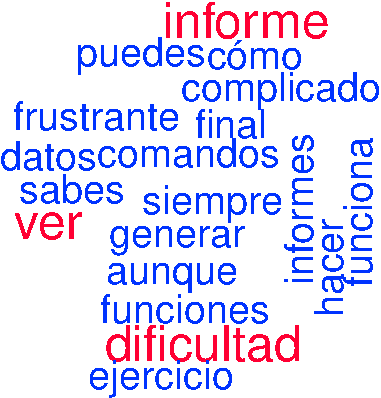
\includegraphics{informe_files/figure-latex/unnamed-chunk-15-1.pdf}

\hypertarget{uxedtem-15-lo-que-muxe1s-me-ha-costado-de-es}{%
\section{\texorpdfstring{Ítem 15: Lo que más me ha costado de
\texttt{R Markdown}
es\ldots{}}{Ítem 15: Lo que más me ha costado de  es\ldots{}}}\label{uxedtem-15-lo-que-muxe1s-me-ha-costado-de-es}}

\begin{Shaded}
\begin{Highlighting}[]
\CommentTok{\# Vector de texto}
\NormalTok{encuesta}\SpecialCharTok{$}\NormalTok{P15}
\end{Highlighting}
\end{Shaded}

\begin{verbatim}
##  [1] "Entender donde buscar cada tipo de test"                                                                                                                                                                                      
##  [2] "trabajar con mi compañero"                                                                                                                                                                                                    
##  [3] "Aprender a hacer todo desde el principio y saber donde está casa cosa."                                                                                                                                                       
##  [4] "Entender la interfaz y los pasos a realizar"                                                                                                                                                                                  
##  [5] "Nada en particular."                                                                                                                                                                                                          
##  [6] "Acostumbrarme en un primer momento "                                                                                                                                                                                          
##  [7] NA                                                                                                                                                                                                                             
##  [8] "Que es un programa informático que es algo que a mi me cuesta personalmente."                                                                                                                                                 
##  [9] NA                                                                                                                                                                                                                             
## [10] "Saber qué hacer con los datos, luego manejarlo en r markdown es bastante fácil"                                                                                                                                               
## [11] "poco, es un programa muy claro e interactivo."                                                                                                                                                                                
## [12] "Aprender que disposición tiene cada opción "                                                                                                                                                                                  
## [13] "Aprender los comandos"                                                                                                                                                                                                        
## [14] "Al principio seguir el ritmo del profesor, pero luego bien."                                                                                                                                                                  
## [15] NA                                                                                                                                                                                                                             
## [16] NA                                                                                                                                                                                                                             
## [17] "Alguna práctica en la que tenía ciertas dudas pero en cuanto eran resueltas no resultaba costoso"                                                                                                                             
## [18] "Al principio cuesta cogerle el truco, pero en la segunda práctica ya lo manejas al 100%."                                                                                                                                     
## [19] "Cambiar cosas dentro de R es un poco confuzo a vecces"                                                                                                                                                                        
## [20] NA                                                                                                                                                                                                                             
## [21] "A voltes no tens clar quin és el arxiu generat si has guardat més coses, pots equivocar-te al pujar l’arxiu a altre lloc."                                                                                                    
## [22] "Guardar l'informe en un arxiu vàlid per a pujar-ho a la tasca."                                                                                                                                                               
## [23] NA                                                                                                                                                                                                                             
## [24] NA                                                                                                                                                                                                                             
## [25] "entendre on he de mirar"                                                                                                                                                                                                      
## [26] "Saber quins tests he d’aplicar en cada exercici"                                                                                                                                                                              
## [27] NA                                                                                                                                                                                                                             
## [28] "Interpretar les dades."                                                                                                                                                                                                       
## [29] NA                                                                                                                                                                                                                             
## [30] NA                                                                                                                                                                                                                             
## [31] "Tobar algunes funcions e interpretar alguns resultats"                                                                                                                                                                        
## [32] NA                                                                                                                                                                                                                             
## [33] NA                                                                                                                                                                                                                             
## [34] "Saber quines opcions en algunes eïnes he de marcar per establir certes condicions a l'hora d'analitzar les dades."                                                                                                            
## [35] NA                                                                                                                                                                                                                             
## [36] NA                                                                                                                                                                                                                             
## [37] "tot"                                                                                                                                                                                                                          
## [38] "Aprendre com es fan alguns procediments o quan hi ha que marcar algunes caselles com que s'ha d'agrupar per grups o lo que siga. De vegades també em costava haver de fer alguns procediments perque no entenia el raonament."
## [39] "certes funcions"                                                                                                                                                                                                              
## [40] "Buscar on he d'anar quan el exercici em demanava alguns gràfics. "                                                                                                                                                            
## [41] " trobar el mètode a executar dins del programa"                                                                                                                                                                               
## [42] "Aprendre a interpretar les dades, sobre tot de les taules de contingència. "                                                                                                                                                  
## [43] "-"                                                                                                                                                                                                                            
## [44] NA                                                                                                                                                                                                                             
## [45] NA                                                                                                                                                                                                                             
## [46] NA                                                                                                                                                                                                                             
## [47] NA
\end{verbatim}

\begin{Shaded}
\begin{Highlighting}[]
\NormalTok{text\_vector }\OtherTok{\textless{}{-}} \FunctionTok{c}\NormalTok{(}
  \StringTok{"Entender dónde buscar cada tipo de test"}\NormalTok{,}
  \StringTok{"Trabajar con mi compañero"}\NormalTok{,}
  \StringTok{"Aprender a hacerlo todo desde el principio y saber dónde está cada cosa"}\NormalTok{,}
  \StringTok{"Entender la interfaz y los pasos a seguir"}\NormalTok{,}
  \StringTok{"Nada en particular"}\NormalTok{,}
  \StringTok{"Acostumbrarme al principio"}\NormalTok{,}
  \ConstantTok{NA}\NormalTok{,}
  \StringTok{"Es un programa informático, lo cual me cuesta personalmente"}\NormalTok{,}
  \ConstantTok{NA}\NormalTok{,}
  \StringTok{"Saber qué hacer con los datos; luego manejarlo en R Markdown es bastante fácil"}\NormalTok{,}
  \StringTok{"Poco, es un programa muy claro e interactivo"}\NormalTok{,}
  \StringTok{"Aprender qué disposición tiene cada opción"}\NormalTok{,}
  \StringTok{"Aprender los comandos"}\NormalTok{,}
  \StringTok{"Al principio seguir el ritmo del profesor, pero luego bien"}\NormalTok{,}
  \ConstantTok{NA}\NormalTok{,}
  \ConstantTok{NA}\NormalTok{,}
  \StringTok{"Alguna práctica en la que tenía ciertas dudas, pero una vez resueltas no resultaba costoso"}\NormalTok{,}
  \StringTok{"Al principio cuesta cogerle el truco, pero en la segunda práctica ya lo manejas al 100\%"}\NormalTok{,}
  \StringTok{"Cambiar cosas dentro de R es un poco confuso a veces"}\NormalTok{,}
  \ConstantTok{NA}\NormalTok{,}
  \StringTok{"A veces no tienes claro cuál es el archivo generado si has guardado más cosas, puedes equivocarte al subir el archivo a otro sitio"}\NormalTok{,}
  \StringTok{"Guardar el informe en un archivo válido para subirlo a la tarea"}\NormalTok{,}
  \ConstantTok{NA}\NormalTok{,}
  \ConstantTok{NA}\NormalTok{,}
  \StringTok{"Entender dónde tengo que mirar"}\NormalTok{,}
  \StringTok{"Saber qué tests aplicar en cada ejercicio"}\NormalTok{,}
  \ConstantTok{NA}\NormalTok{,}
  \StringTok{"Interpretar los datos"}\NormalTok{,}
  \ConstantTok{NA}\NormalTok{,}
  \ConstantTok{NA}\NormalTok{,}
  \StringTok{"Encontrar algunas funciones e interpretar algunos resultados"}\NormalTok{,}
  \ConstantTok{NA}\NormalTok{,}
  \ConstantTok{NA}\NormalTok{,}
  \StringTok{"Saber qué opciones marcar en algunas herramientas para establecer ciertas condiciones al analizar los datos"}\NormalTok{,}
  \ConstantTok{NA}\NormalTok{,}
  \ConstantTok{NA}\NormalTok{,}
  \StringTok{"Todo"}\NormalTok{,}
  \StringTok{"Aprender cómo se hacen algunos procedimientos o cuándo hay que marcar algunas casillas como agrupar por grupos, o lo que sea. A veces también me costaba hacer ciertos procedimientos porque no entendía el razonamiento"}\NormalTok{,}
  \StringTok{"Ciertas funciones"}\NormalTok{,}
  \StringTok{"Buscar a dónde ir cuando el ejercicio pedía ciertos gráficos"}\NormalTok{,}
  \StringTok{"Encontrar el método a ejecutar dentro del programa"}\NormalTok{,}
  \StringTok{"Aprender a interpretar los datos, sobre todo de las tablas de contingencia"}\NormalTok{,}
  \ConstantTok{NA}\NormalTok{,}
  \ConstantTok{NA}\NormalTok{,}
  \ConstantTok{NA}\NormalTok{,}
  \ConstantTok{NA}\NormalTok{,}
  \ConstantTok{NA}
\NormalTok{)}

\CommentTok{\# Convierte a un corpus}
\NormalTok{corpus }\OtherTok{\textless{}{-}} \FunctionTok{Corpus}\NormalTok{(}\FunctionTok{VectorSource}\NormalTok{(text\_vector))}

\CommentTok{\# Limpieza básica del texto}
\NormalTok{corpus }\OtherTok{\textless{}{-}} \FunctionTok{tm\_map}\NormalTok{(corpus, removePunctuation)                    }\CommentTok{\# elimina puntuación}
\end{Highlighting}
\end{Shaded}

\begin{verbatim}
## Warning in tm_map.SimpleCorpus(corpus, removePunctuation): transformation drops
## documents
\end{verbatim}

\begin{Shaded}
\begin{Highlighting}[]
\NormalTok{corpus }\OtherTok{\textless{}{-}} \FunctionTok{tm\_map}\NormalTok{(corpus, }\FunctionTok{content\_transformer}\NormalTok{(tolower))         }\CommentTok{\# a minúsculas}
\end{Highlighting}
\end{Shaded}

\begin{verbatim}
## Warning in tm_map.SimpleCorpus(corpus, content_transformer(tolower)):
## transformation drops documents
\end{verbatim}

\begin{Shaded}
\begin{Highlighting}[]
\NormalTok{corpus }\OtherTok{\textless{}{-}} \FunctionTok{tm\_map}\NormalTok{(corpus, removeNumbers)                        }\CommentTok{\# elimina números}
\end{Highlighting}
\end{Shaded}

\begin{verbatim}
## Warning in tm_map.SimpleCorpus(corpus, removeNumbers): transformation drops
## documents
\end{verbatim}

\begin{Shaded}
\begin{Highlighting}[]
\NormalTok{corpus }\OtherTok{\textless{}{-}} \FunctionTok{tm\_map}\NormalTok{(corpus, stripWhitespace)                      }\CommentTok{\# elimina muchos espacios}
\end{Highlighting}
\end{Shaded}

\begin{verbatim}
## Warning in tm_map.SimpleCorpus(corpus, stripWhitespace): transformation drops
## documents
\end{verbatim}

\begin{Shaded}
\begin{Highlighting}[]
\NormalTok{corpus }\OtherTok{\textless{}{-}} \FunctionTok{tm\_map}\NormalTok{(corpus, removeWords, }\FunctionTok{stopwords}\NormalTok{(}\StringTok{"spanish"}\NormalTok{))    }\CommentTok{\# elimina stopwords en español}
\end{Highlighting}
\end{Shaded}

\begin{verbatim}
## Warning in tm_map.SimpleCorpus(corpus, removeWords, stopwords("spanish")):
## transformation drops documents
\end{verbatim}

\begin{Shaded}
\begin{Highlighting}[]
\CommentTok{\# Crear matriz de términos}
\NormalTok{tdm }\OtherTok{\textless{}{-}} \FunctionTok{TermDocumentMatrix}\NormalTok{(corpus)}
\NormalTok{m }\OtherTok{\textless{}{-}} \FunctionTok{as.matrix}\NormalTok{(tdm)}
\NormalTok{word\_freqs }\OtherTok{\textless{}{-}} \FunctionTok{sort}\NormalTok{(}\FunctionTok{rowSums}\NormalTok{(m), }\AttributeTok{decreasing =} \ConstantTok{TRUE}\NormalTok{)}

\CommentTok{\# Dibujar la nube}
\FunctionTok{par}\NormalTok{(}\AttributeTok{mar =} \FunctionTok{c}\NormalTok{(}\DecValTok{1}\NormalTok{, }\DecValTok{1}\NormalTok{, }\DecValTok{1}\NormalTok{, }\DecValTok{1}\NormalTok{))}
\FunctionTok{wordcloud}\NormalTok{(}\FunctionTok{names}\NormalTok{(word\_freqs), }\AttributeTok{scale =} \FunctionTok{c}\NormalTok{(}\DecValTok{2}\NormalTok{, }\FloatTok{0.75}\NormalTok{), word\_freqs, }\AttributeTok{min.freq =} \DecValTok{2}\NormalTok{, }
          \AttributeTok{colors =} \FunctionTok{rainbow}\NormalTok{(}\DecValTok{30}\NormalTok{))}
\end{Highlighting}
\end{Shaded}

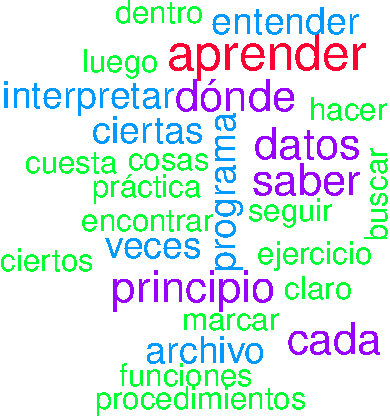
\includegraphics{informe_files/figure-latex/unnamed-chunk-16-1.pdf}

\hypertarget{uxedtem-16-cuxf3mo-mejoraruxedas-las-clases-en-el-uso-de}{%
\section{\texorpdfstring{Ítem 16: ¿Cómo mejorarías las clases en el uso
de
\texttt{R Markdown}?}{Ítem 16: ¿Cómo mejorarías las clases en el uso de ?}}\label{uxedtem-16-cuxf3mo-mejoraruxedas-las-clases-en-el-uso-de}}

\begin{Shaded}
\begin{Highlighting}[]
\CommentTok{\# Vector de texto}
\NormalTok{encuesta}\SpecialCharTok{$}\NormalTok{P16}
\end{Highlighting}
\end{Shaded}

\begin{verbatim}
##  [1] "No tengo ninguna aportación"                                                                                                                                                                                                                                                                                                                                                                        
##  [2] "no sé"                                                                                                                                                                                                                                                                                                                                                                                              
##  [3] "Quizás hacerlas en grupos de menos personas para que sea más fácil seguir la clase."                                                                                                                                                                                                                                                                                                                
##  [4] "Concretando en cada parte más"                                                                                                                                                                                                                                                                                                                                                                      
##  [5] "Incluir en los guiones de las prácticas las claves necesarias para usarlo, como ordenarlo y luego guardarlo en ambos formatos, ya que nos solemos olvidar de como hacerlo. "                                                                                                                                                                                                                        
##  [6] "No sé, me han parecido adecuadas y comprensibles."                                                                                                                                                                                                                                                                                                                                                  
##  [7] NA                                                                                                                                                                                                                                                                                                                                                                                                   
##  [8] "Explicando todos los pasos a seguir, de forma más clara."                                                                                                                                                                                                                                                                                                                                           
##  [9] NA                                                                                                                                                                                                                                                                                                                                                                                                   
## [10] NA                                                                                                                                                                                                                                                                                                                                                                                                   
## [11] "pocas cosas podrían ser mejorables, a lo mejor, tener una pestaña de tiempo real del informe."                                                                                                                                                                                                                                                                                                      
## [12] "Aprender en grupos más reducidos"                                                                                                                                                                                                                                                                                                                                                                   
## [13] "No lo sé, yo las he considerado bastante buenas la verdad "                                                                                                                                                                                                                                                                                                                                         
## [14] "Haría ejercicios más completos, en el sentido de que se pudieran usar más funciones del programa y promovería el uso individual de la herramienta, no todo el mundo aprende al mismo ritmo ni se va a quedar con todo de la misma manera, hay días que es difícil seguir el ritmo y otros que se hacen muy lentos. También añadiría entregas opcionales de las tareas para incentivar este trabajo."
## [15] "En general, personalmente, las he visto bastante bien organizadas y fáciles de seguir. "                                                                                                                                                                                                                                                                                                            
## [16] NA                                                                                                                                                                                                                                                                                                                                                                                                   
## [17] "No considero que haya mejoras a hacer :)"                                                                                                                                                                                                                                                                                                                                                           
## [18] NA                                                                                                                                                                                                                                                                                                                                                                                                   
## [19] NA                                                                                                                                                                                                                                                                                                                                                                                                   
## [20] "Ve más despacio y haz las cosas con más detalle"                                                                                                                                                                                                                                                                                                                                                    
## [21] "Posaria una guia amb totes les coses que es pot fer, i com ordenar els aparts al r Markdown."                                                                                                                                                                                                                                                                                                       
## [22] "Potser posaria menys exercicis (o més hores) ja que, cap al final de les sessions anàvem bastant agobiats per la falta de temps; no era capaç d'atendre la resolució de l'exercici, fer-la al R i escriure-la. "                                                                                                                                                                                    
## [23] NA                                                                                                                                                                                                                                                                                                                                                                                                   
## [24] NA                                                                                                                                                                                                                                                                                                                                                                                                   
## [25] "enfocament distint de les classes"                                                                                                                                                                                                                                                                                                                                                                  
## [26] "Explicant un poc els exercicis per poder arribar a saber de quin tipus de mostra es tracta i quins tests s’han de fer"                                                                                                                                                                                                                                                                              
## [27] NA                                                                                                                                                                                                                                                                                                                                                                                                   
## [28] "Centrar les explicacions un poc més en la navegació a les diferents pestanyes de l'aplicació."                                                                                                                                                                                                                                                                                                      
## [29] NA                                                                                                                                                                                                                                                                                                                                                                                                   
## [30] NA                                                                                                                                                                                                                                                                                                                                                                                                   
## [31] "Tot bé"                                                                                                                                                                                                                                                                                                                                                                                             
## [32] NA                                                                                                                                                                                                                                                                                                                                                                                                   
## [33] NA                                                                                                                                                                                                                                                                                                                                                                                                   
## [34] "Una major relació entre com serà l'examen amb la metodología de les pràctiques."                                                                                                                                                                                                                                                                                                                    
## [35] "Explicant més tetalladament el seu funcionament"                                                                                                                                                                                                                                                                                                                                                    
## [36] NA                                                                                                                                                                                                                                                                                                                                                                                                   
## [37] "utilizando un programa mas facil"                                                                                                                                                                                                                                                                                                                                                                   
## [38] "A lo millor anar un miqueta més lent, ja que havia vegades que algunes preguntes no quedaven clares perque haviem de fer molts exercicis. "                                                                                                                                                                                                                                                         
## [39] NA                                                                                                                                                                                                                                                                                                                                                                                                   
## [40] "Ir un poc més aspai, perquè hi havia vegades que em perdia"                                                                                                                                                                                                                                                                                                                                         
## [41] "No sabria dir. "                                                                                                                                                                                                                                                                                                                                                                                    
## [42] "Crec que estan ben organitzades. "                                                                                                                                                                                                                                                                                                                                                                  
## [43] "-"                                                                                                                                                                                                                                                                                                                                                                                                  
## [44] NA                                                                                                                                                                                                                                                                                                                                                                                                   
## [45] NA                                                                                                                                                                                                                                                                                                                                                                                                   
## [46] NA                                                                                                                                                                                                                                                                                                                                                                                                   
## [47] NA
\end{verbatim}

\begin{Shaded}
\begin{Highlighting}[]
\NormalTok{text\_vector }\OtherTok{\textless{}{-}} \FunctionTok{c}\NormalTok{(}
  \StringTok{"No tengo ninguna aportación"}\NormalTok{,}
  \StringTok{"No sé"}\NormalTok{,}
  \StringTok{"Quizás hacerlas en grupos más pequeños para que sea más fácil seguir la clase"}\NormalTok{,}
  \StringTok{"Concretar más en cada parte"}\NormalTok{,}
  \StringTok{"Incluir en los guiones de las prácticas las claves necesarias para usarlo, como ordenarlo y luego guardarlo en ambos formatos, ya que solemos olvidar cómo hacerlo"}\NormalTok{,}
  \StringTok{"No sé, me han parecido adecuadas y comprensibles"}\NormalTok{,}
  \ConstantTok{NA}\NormalTok{,}
  \StringTok{"Explicar todos los pasos a seguir de forma más clara"}\NormalTok{,}
  \ConstantTok{NA}\NormalTok{,}
  \ConstantTok{NA}\NormalTok{,}
  \StringTok{"Pocas cosas podrían ser mejorables; quizás tener una pestaña de tiempo real del informe"}\NormalTok{,}
  \StringTok{"Aprender en grupos más reducidos"}\NormalTok{,}
  \StringTok{"No lo sé, me han parecido bastante buenas, la verdad"}\NormalTok{,}
  \StringTok{"Haría ejercicios más completos, que permitieran usar más funciones del programa, y promovería el uso individual de la herramienta. No todo el mundo aprende al mismo ritmo ni se quedará con todo igual; hay días que es difícil seguir el ritmo y otros que se hacen muy lentos. También añadiría entregas opcionales para incentivar el trabajo"}\NormalTok{,}
  \StringTok{"En general, personalmente, las he visto bastante bien organizadas y fáciles de seguir"}\NormalTok{,}
  \ConstantTok{NA}\NormalTok{,}
  \StringTok{"No considero que haya mejoras que hacer :)"}\NormalTok{,}
  \ConstantTok{NA}\NormalTok{,}
  \ConstantTok{NA}\NormalTok{,}
  \StringTok{"Ir más despacio y hacer las cosas con más detalle"}\NormalTok{,}
  \StringTok{"Pondría una guía con todas las cosas que se pueden hacer y cómo ordenar los apartados en el R Markdown"}\NormalTok{,}
  \StringTok{"Quizás pondría menos ejercicios (o más tiempo), ya que al final de las sesiones íbamos bastante agobiados por la falta de tiempo; no era capaz de atender a la resolución del ejercicio, hacerlo en R y escribirlo"}\NormalTok{,}
  \ConstantTok{NA}\NormalTok{,}
  \ConstantTok{NA}\NormalTok{,}
  \StringTok{"Un enfoque distinto en las clases"}\NormalTok{,}
  \StringTok{"Explicar un poco los ejercicios para saber de qué tipo de muestra se trata y qué tests hay que hacer"}\NormalTok{,}
  \ConstantTok{NA}\NormalTok{,}
  \StringTok{"Centrar las explicaciones un poco más en la navegación por las distintas pestañas de la aplicación"}\NormalTok{,}
  \ConstantTok{NA}\NormalTok{,}
  \ConstantTok{NA}\NormalTok{,}
  \StringTok{"Todo bien"}\NormalTok{,}
  \ConstantTok{NA}\NormalTok{,}
  \ConstantTok{NA}\NormalTok{,}
  \StringTok{"Una mayor relación entre cómo será el examen y la metodología de las prácticas"}\NormalTok{,}
  \StringTok{"Explicar más detalladamente su funcionamiento"}\NormalTok{,}
  \ConstantTok{NA}\NormalTok{,}
  \StringTok{"Utilizar un programa más fácil"}\NormalTok{,}
  \StringTok{"Quizás ir un poco más lento, ya que a veces algunas preguntas no quedaban claras porque había que hacer muchos ejercicios"}\NormalTok{,}
  \ConstantTok{NA}\NormalTok{,}
  \StringTok{"Ir un poco más despacio, porque a veces me perdía"}\NormalTok{,}
  \StringTok{"No sabría decir"}\NormalTok{,}
  \StringTok{"Creo que están bien organizadas"}\NormalTok{,}
  \ConstantTok{NA}\NormalTok{,}
  \ConstantTok{NA}\NormalTok{,}
  \ConstantTok{NA}\NormalTok{,}
  \ConstantTok{NA}\NormalTok{,}
  \ConstantTok{NA}
\NormalTok{)}

\CommentTok{\# Convierte a un corpus}
\NormalTok{corpus }\OtherTok{\textless{}{-}} \FunctionTok{Corpus}\NormalTok{(}\FunctionTok{VectorSource}\NormalTok{(text\_vector))}

\CommentTok{\# Limpieza básica del texto}
\NormalTok{corpus }\OtherTok{\textless{}{-}} \FunctionTok{tm\_map}\NormalTok{(corpus, removePunctuation)                    }\CommentTok{\# elimina puntuación}
\end{Highlighting}
\end{Shaded}

\begin{verbatim}
## Warning in tm_map.SimpleCorpus(corpus, removePunctuation): transformation drops
## documents
\end{verbatim}

\begin{Shaded}
\begin{Highlighting}[]
\NormalTok{corpus }\OtherTok{\textless{}{-}} \FunctionTok{tm\_map}\NormalTok{(corpus, }\FunctionTok{content\_transformer}\NormalTok{(tolower))         }\CommentTok{\# a minúsculas}
\end{Highlighting}
\end{Shaded}

\begin{verbatim}
## Warning in tm_map.SimpleCorpus(corpus, content_transformer(tolower)):
## transformation drops documents
\end{verbatim}

\begin{Shaded}
\begin{Highlighting}[]
\NormalTok{corpus }\OtherTok{\textless{}{-}} \FunctionTok{tm\_map}\NormalTok{(corpus, removeNumbers)                        }\CommentTok{\# elimina números}
\end{Highlighting}
\end{Shaded}

\begin{verbatim}
## Warning in tm_map.SimpleCorpus(corpus, removeNumbers): transformation drops
## documents
\end{verbatim}

\begin{Shaded}
\begin{Highlighting}[]
\NormalTok{corpus }\OtherTok{\textless{}{-}} \FunctionTok{tm\_map}\NormalTok{(corpus, stripWhitespace)                      }\CommentTok{\# elimina muchos espacios}
\end{Highlighting}
\end{Shaded}

\begin{verbatim}
## Warning in tm_map.SimpleCorpus(corpus, stripWhitespace): transformation drops
## documents
\end{verbatim}

\begin{Shaded}
\begin{Highlighting}[]
\NormalTok{corpus }\OtherTok{\textless{}{-}} \FunctionTok{tm\_map}\NormalTok{(corpus, removeWords, }\FunctionTok{stopwords}\NormalTok{(}\StringTok{"spanish"}\NormalTok{))    }\CommentTok{\# elimina stopwords en español}
\end{Highlighting}
\end{Shaded}

\begin{verbatim}
## Warning in tm_map.SimpleCorpus(corpus, removeWords, stopwords("spanish")):
## transformation drops documents
\end{verbatim}

\begin{Shaded}
\begin{Highlighting}[]
\CommentTok{\# Crear matriz de términos}
\NormalTok{tdm }\OtherTok{\textless{}{-}} \FunctionTok{TermDocumentMatrix}\NormalTok{(corpus)}
\NormalTok{m }\OtherTok{\textless{}{-}} \FunctionTok{as.matrix}\NormalTok{(tdm)}
\NormalTok{word\_freqs }\OtherTok{\textless{}{-}} \FunctionTok{sort}\NormalTok{(}\FunctionTok{rowSums}\NormalTok{(m), }\AttributeTok{decreasing =} \ConstantTok{TRUE}\NormalTok{)}

\CommentTok{\# Dibujar la nube}
\FunctionTok{par}\NormalTok{(}\AttributeTok{mar =} \FunctionTok{c}\NormalTok{(}\DecValTok{1}\NormalTok{, }\DecValTok{1}\NormalTok{, }\DecValTok{1}\NormalTok{, }\DecValTok{1}\NormalTok{))}
\FunctionTok{wordcloud}\NormalTok{(}\FunctionTok{names}\NormalTok{(word\_freqs), }\AttributeTok{scale =} \FunctionTok{c}\NormalTok{(}\DecValTok{2}\NormalTok{, }\FloatTok{0.75}\NormalTok{), word\_freqs, }\AttributeTok{min.freq =} \DecValTok{2}\NormalTok{, }
          \AttributeTok{colors =} \FunctionTok{rainbow}\NormalTok{(}\DecValTok{30}\NormalTok{))}
\end{Highlighting}
\end{Shaded}

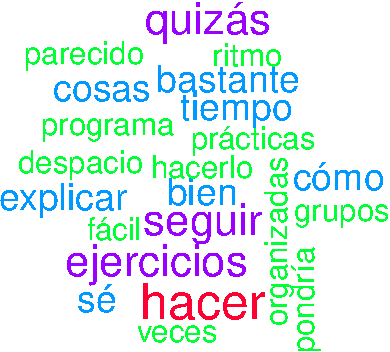
\includegraphics{informe_files/figure-latex/unnamed-chunk-17-1.pdf}

\end{document}
